\documentclass[11pt]{article}

    \usepackage[breakable]{tcolorbox}
    \usepackage{parskip} % Stop auto-indenting (to mimic markdown behaviour)
    
    \usepackage{iftex}
    \ifPDFTeX
    	\usepackage[T1]{fontenc}
    	\usepackage{mathpazo}
    \else
    	\usepackage{fontspec}
    \fi

    % Basic figure setup, for now with no caption control since it's done
    % automatically by Pandoc (which extracts ![](path) syntax from Markdown).
    \usepackage{graphicx}
    % Maintain compatibility with old templates. Remove in nbconvert 6.0
    \let\Oldincludegraphics\includegraphics
    % Ensure that by default, figures have no caption (until we provide a
    % proper Figure object with a Caption API and a way to capture that
    % in the conversion process - todo).
    \usepackage{caption}
    \DeclareCaptionFormat{nocaption}{}
    \captionsetup{format=nocaption,aboveskip=0pt,belowskip=0pt}

    \usepackage[Export]{adjustbox} % Used to constrain images to a maximum size
    \adjustboxset{max size={0.9\linewidth}{0.9\paperheight}}
    \usepackage{float}
    \floatplacement{figure}{H} % forces figures to be placed at the correct location
    \usepackage{xcolor} % Allow colors to be defined
    \usepackage{enumerate} % Needed for markdown enumerations to work
    \usepackage{geometry} % Used to adjust the document margins
    \usepackage{amsmath} % Equations
    \usepackage{amssymb} % Equations
    \usepackage{textcomp} % defines textquotesingle
    % Hack from http://tex.stackexchange.com/a/47451/13684:
    \AtBeginDocument{%
        \def\PYZsq{\textquotesingle}% Upright quotes in Pygmentized code
    }
    \usepackage{upquote} % Upright quotes for verbatim code
    \usepackage{eurosym} % defines \euro
    \usepackage[mathletters]{ucs} % Extended unicode (utf-8) support
    \usepackage{fancyvrb} % verbatim replacement that allows latex
    \usepackage{grffile} % extends the file name processing of package graphics 
                         % to support a larger range
    \makeatletter % fix for grffile with XeLaTeX
    \def\Gread@@xetex#1{%
      \IfFileExists{"\Gin@base".bb}%
      {\Gread@eps{\Gin@base.bb}}%
      {\Gread@@xetex@aux#1}%
    }
    \makeatother

    % The hyperref package gives us a pdf with properly built
    % internal navigation ('pdf bookmarks' for the table of contents,
    % internal cross-reference links, web links for URLs, etc.)
    \usepackage{hyperref}
    % The default LaTeX title has an obnoxious amount of whitespace. By default,
    % titling removes some of it. It also provides customization options.
    \usepackage{titling}
    \usepackage{longtable} % longtable support required by pandoc >1.10
    \usepackage{booktabs}  % table support for pandoc > 1.12.2
    \usepackage[inline]{enumitem} % IRkernel/repr support (it uses the enumerate* environment)
    \usepackage[normalem]{ulem} % ulem is needed to support strikethroughs (\sout)
                                % normalem makes italics be italics, not underlines
    \usepackage{mathrsfs}
    

    
    % Colors for the hyperref package
    \definecolor{urlcolor}{rgb}{0,.145,.698}
    \definecolor{linkcolor}{rgb}{.71,0.21,0.01}
    \definecolor{citecolor}{rgb}{.12,.54,.11}

    % ANSI colors
    \definecolor{ansi-black}{HTML}{3E424D}
    \definecolor{ansi-black-intense}{HTML}{282C36}
    \definecolor{ansi-red}{HTML}{E75C58}
    \definecolor{ansi-red-intense}{HTML}{B22B31}
    \definecolor{ansi-green}{HTML}{00A250}
    \definecolor{ansi-green-intense}{HTML}{007427}
    \definecolor{ansi-yellow}{HTML}{DDB62B}
    \definecolor{ansi-yellow-intense}{HTML}{B27D12}
    \definecolor{ansi-blue}{HTML}{208FFB}
    \definecolor{ansi-blue-intense}{HTML}{0065CA}
    \definecolor{ansi-magenta}{HTML}{D160C4}
    \definecolor{ansi-magenta-intense}{HTML}{A03196}
    \definecolor{ansi-cyan}{HTML}{60C6C8}
    \definecolor{ansi-cyan-intense}{HTML}{258F8F}
    \definecolor{ansi-white}{HTML}{C5C1B4}
    \definecolor{ansi-white-intense}{HTML}{A1A6B2}
    \definecolor{ansi-default-inverse-fg}{HTML}{FFFFFF}
    \definecolor{ansi-default-inverse-bg}{HTML}{000000}

    % commands and environments needed by pandoc snippets
    % extracted from the output of `pandoc -s`
    \providecommand{\tightlist}{%
      \setlength{\itemsep}{0pt}\setlength{\parskip}{0pt}}
    \DefineVerbatimEnvironment{Highlighting}{Verbatim}{commandchars=\\\{\}}
    % Add ',fontsize=\small' for more characters per line
    \newenvironment{Shaded}{}{}
    \newcommand{\KeywordTok}[1]{\textcolor[rgb]{0.00,0.44,0.13}{\textbf{{#1}}}}
    \newcommand{\DataTypeTok}[1]{\textcolor[rgb]{0.56,0.13,0.00}{{#1}}}
    \newcommand{\DecValTok}[1]{\textcolor[rgb]{0.25,0.63,0.44}{{#1}}}
    \newcommand{\BaseNTok}[1]{\textcolor[rgb]{0.25,0.63,0.44}{{#1}}}
    \newcommand{\FloatTok}[1]{\textcolor[rgb]{0.25,0.63,0.44}{{#1}}}
    \newcommand{\CharTok}[1]{\textcolor[rgb]{0.25,0.44,0.63}{{#1}}}
    \newcommand{\StringTok}[1]{\textcolor[rgb]{0.25,0.44,0.63}{{#1}}}
    \newcommand{\CommentTok}[1]{\textcolor[rgb]{0.38,0.63,0.69}{\textit{{#1}}}}
    \newcommand{\OtherTok}[1]{\textcolor[rgb]{0.00,0.44,0.13}{{#1}}}
    \newcommand{\AlertTok}[1]{\textcolor[rgb]{1.00,0.00,0.00}{\textbf{{#1}}}}
    \newcommand{\FunctionTok}[1]{\textcolor[rgb]{0.02,0.16,0.49}{{#1}}}
    \newcommand{\RegionMarkerTok}[1]{{#1}}
    \newcommand{\ErrorTok}[1]{\textcolor[rgb]{1.00,0.00,0.00}{\textbf{{#1}}}}
    \newcommand{\NormalTok}[1]{{#1}}
    
    % Additional commands for more recent versions of Pandoc
    \newcommand{\ConstantTok}[1]{\textcolor[rgb]{0.53,0.00,0.00}{{#1}}}
    \newcommand{\SpecialCharTok}[1]{\textcolor[rgb]{0.25,0.44,0.63}{{#1}}}
    \newcommand{\VerbatimStringTok}[1]{\textcolor[rgb]{0.25,0.44,0.63}{{#1}}}
    \newcommand{\SpecialStringTok}[1]{\textcolor[rgb]{0.73,0.40,0.53}{{#1}}}
    \newcommand{\ImportTok}[1]{{#1}}
    \newcommand{\DocumentationTok}[1]{\textcolor[rgb]{0.73,0.13,0.13}{\textit{{#1}}}}
    \newcommand{\AnnotationTok}[1]{\textcolor[rgb]{0.38,0.63,0.69}{\textbf{\textit{{#1}}}}}
    \newcommand{\CommentVarTok}[1]{\textcolor[rgb]{0.38,0.63,0.69}{\textbf{\textit{{#1}}}}}
    \newcommand{\VariableTok}[1]{\textcolor[rgb]{0.10,0.09,0.49}{{#1}}}
    \newcommand{\ControlFlowTok}[1]{\textcolor[rgb]{0.00,0.44,0.13}{\textbf{{#1}}}}
    \newcommand{\OperatorTok}[1]{\textcolor[rgb]{0.40,0.40,0.40}{{#1}}}
    \newcommand{\BuiltInTok}[1]{{#1}}
    \newcommand{\ExtensionTok}[1]{{#1}}
    \newcommand{\PreprocessorTok}[1]{\textcolor[rgb]{0.74,0.48,0.00}{{#1}}}
    \newcommand{\AttributeTok}[1]{\textcolor[rgb]{0.49,0.56,0.16}{{#1}}}
    \newcommand{\InformationTok}[1]{\textcolor[rgb]{0.38,0.63,0.69}{\textbf{\textit{{#1}}}}}
    \newcommand{\WarningTok}[1]{\textcolor[rgb]{0.38,0.63,0.69}{\textbf{\textit{{#1}}}}}
    
    
    % Define a nice break command that doesn't care if a line doesn't already
    % exist.
    \def\br{\hspace*{\fill} \\* }
    % Math Jax compatibility definitions
    \def\gt{>}
    \def\lt{<}
    \let\Oldtex\TeX
    \let\Oldlatex\LaTeX
    \renewcommand{\TeX}{\textrm{\Oldtex}}
    \renewcommand{\LaTeX}{\textrm{\Oldlatex}}
    % Document parameters
    % Document title
    \title{face-verification-recognition}
    
    
    
    
    
% Pygments definitions
\makeatletter
\def\PY@reset{\let\PY@it=\relax \let\PY@bf=\relax%
    \let\PY@ul=\relax \let\PY@tc=\relax%
    \let\PY@bc=\relax \let\PY@ff=\relax}
\def\PY@tok#1{\csname PY@tok@#1\endcsname}
\def\PY@toks#1+{\ifx\relax#1\empty\else%
    \PY@tok{#1}\expandafter\PY@toks\fi}
\def\PY@do#1{\PY@bc{\PY@tc{\PY@ul{%
    \PY@it{\PY@bf{\PY@ff{#1}}}}}}}
\def\PY#1#2{\PY@reset\PY@toks#1+\relax+\PY@do{#2}}

\expandafter\def\csname PY@tok@w\endcsname{\def\PY@tc##1{\textcolor[rgb]{0.73,0.73,0.73}{##1}}}
\expandafter\def\csname PY@tok@c\endcsname{\let\PY@it=\textit\def\PY@tc##1{\textcolor[rgb]{0.25,0.50,0.50}{##1}}}
\expandafter\def\csname PY@tok@cp\endcsname{\def\PY@tc##1{\textcolor[rgb]{0.74,0.48,0.00}{##1}}}
\expandafter\def\csname PY@tok@k\endcsname{\let\PY@bf=\textbf\def\PY@tc##1{\textcolor[rgb]{0.00,0.50,0.00}{##1}}}
\expandafter\def\csname PY@tok@kp\endcsname{\def\PY@tc##1{\textcolor[rgb]{0.00,0.50,0.00}{##1}}}
\expandafter\def\csname PY@tok@kt\endcsname{\def\PY@tc##1{\textcolor[rgb]{0.69,0.00,0.25}{##1}}}
\expandafter\def\csname PY@tok@o\endcsname{\def\PY@tc##1{\textcolor[rgb]{0.40,0.40,0.40}{##1}}}
\expandafter\def\csname PY@tok@ow\endcsname{\let\PY@bf=\textbf\def\PY@tc##1{\textcolor[rgb]{0.67,0.13,1.00}{##1}}}
\expandafter\def\csname PY@tok@nb\endcsname{\def\PY@tc##1{\textcolor[rgb]{0.00,0.50,0.00}{##1}}}
\expandafter\def\csname PY@tok@nf\endcsname{\def\PY@tc##1{\textcolor[rgb]{0.00,0.00,1.00}{##1}}}
\expandafter\def\csname PY@tok@nc\endcsname{\let\PY@bf=\textbf\def\PY@tc##1{\textcolor[rgb]{0.00,0.00,1.00}{##1}}}
\expandafter\def\csname PY@tok@nn\endcsname{\let\PY@bf=\textbf\def\PY@tc##1{\textcolor[rgb]{0.00,0.00,1.00}{##1}}}
\expandafter\def\csname PY@tok@ne\endcsname{\let\PY@bf=\textbf\def\PY@tc##1{\textcolor[rgb]{0.82,0.25,0.23}{##1}}}
\expandafter\def\csname PY@tok@nv\endcsname{\def\PY@tc##1{\textcolor[rgb]{0.10,0.09,0.49}{##1}}}
\expandafter\def\csname PY@tok@no\endcsname{\def\PY@tc##1{\textcolor[rgb]{0.53,0.00,0.00}{##1}}}
\expandafter\def\csname PY@tok@nl\endcsname{\def\PY@tc##1{\textcolor[rgb]{0.63,0.63,0.00}{##1}}}
\expandafter\def\csname PY@tok@ni\endcsname{\let\PY@bf=\textbf\def\PY@tc##1{\textcolor[rgb]{0.60,0.60,0.60}{##1}}}
\expandafter\def\csname PY@tok@na\endcsname{\def\PY@tc##1{\textcolor[rgb]{0.49,0.56,0.16}{##1}}}
\expandafter\def\csname PY@tok@nt\endcsname{\let\PY@bf=\textbf\def\PY@tc##1{\textcolor[rgb]{0.00,0.50,0.00}{##1}}}
\expandafter\def\csname PY@tok@nd\endcsname{\def\PY@tc##1{\textcolor[rgb]{0.67,0.13,1.00}{##1}}}
\expandafter\def\csname PY@tok@s\endcsname{\def\PY@tc##1{\textcolor[rgb]{0.73,0.13,0.13}{##1}}}
\expandafter\def\csname PY@tok@sd\endcsname{\let\PY@it=\textit\def\PY@tc##1{\textcolor[rgb]{0.73,0.13,0.13}{##1}}}
\expandafter\def\csname PY@tok@si\endcsname{\let\PY@bf=\textbf\def\PY@tc##1{\textcolor[rgb]{0.73,0.40,0.53}{##1}}}
\expandafter\def\csname PY@tok@se\endcsname{\let\PY@bf=\textbf\def\PY@tc##1{\textcolor[rgb]{0.73,0.40,0.13}{##1}}}
\expandafter\def\csname PY@tok@sr\endcsname{\def\PY@tc##1{\textcolor[rgb]{0.73,0.40,0.53}{##1}}}
\expandafter\def\csname PY@tok@ss\endcsname{\def\PY@tc##1{\textcolor[rgb]{0.10,0.09,0.49}{##1}}}
\expandafter\def\csname PY@tok@sx\endcsname{\def\PY@tc##1{\textcolor[rgb]{0.00,0.50,0.00}{##1}}}
\expandafter\def\csname PY@tok@m\endcsname{\def\PY@tc##1{\textcolor[rgb]{0.40,0.40,0.40}{##1}}}
\expandafter\def\csname PY@tok@gh\endcsname{\let\PY@bf=\textbf\def\PY@tc##1{\textcolor[rgb]{0.00,0.00,0.50}{##1}}}
\expandafter\def\csname PY@tok@gu\endcsname{\let\PY@bf=\textbf\def\PY@tc##1{\textcolor[rgb]{0.50,0.00,0.50}{##1}}}
\expandafter\def\csname PY@tok@gd\endcsname{\def\PY@tc##1{\textcolor[rgb]{0.63,0.00,0.00}{##1}}}
\expandafter\def\csname PY@tok@gi\endcsname{\def\PY@tc##1{\textcolor[rgb]{0.00,0.63,0.00}{##1}}}
\expandafter\def\csname PY@tok@gr\endcsname{\def\PY@tc##1{\textcolor[rgb]{1.00,0.00,0.00}{##1}}}
\expandafter\def\csname PY@tok@ge\endcsname{\let\PY@it=\textit}
\expandafter\def\csname PY@tok@gs\endcsname{\let\PY@bf=\textbf}
\expandafter\def\csname PY@tok@gp\endcsname{\let\PY@bf=\textbf\def\PY@tc##1{\textcolor[rgb]{0.00,0.00,0.50}{##1}}}
\expandafter\def\csname PY@tok@go\endcsname{\def\PY@tc##1{\textcolor[rgb]{0.53,0.53,0.53}{##1}}}
\expandafter\def\csname PY@tok@gt\endcsname{\def\PY@tc##1{\textcolor[rgb]{0.00,0.27,0.87}{##1}}}
\expandafter\def\csname PY@tok@err\endcsname{\def\PY@bc##1{\setlength{\fboxsep}{0pt}\fcolorbox[rgb]{1.00,0.00,0.00}{1,1,1}{\strut ##1}}}
\expandafter\def\csname PY@tok@kc\endcsname{\let\PY@bf=\textbf\def\PY@tc##1{\textcolor[rgb]{0.00,0.50,0.00}{##1}}}
\expandafter\def\csname PY@tok@kd\endcsname{\let\PY@bf=\textbf\def\PY@tc##1{\textcolor[rgb]{0.00,0.50,0.00}{##1}}}
\expandafter\def\csname PY@tok@kn\endcsname{\let\PY@bf=\textbf\def\PY@tc##1{\textcolor[rgb]{0.00,0.50,0.00}{##1}}}
\expandafter\def\csname PY@tok@kr\endcsname{\let\PY@bf=\textbf\def\PY@tc##1{\textcolor[rgb]{0.00,0.50,0.00}{##1}}}
\expandafter\def\csname PY@tok@bp\endcsname{\def\PY@tc##1{\textcolor[rgb]{0.00,0.50,0.00}{##1}}}
\expandafter\def\csname PY@tok@fm\endcsname{\def\PY@tc##1{\textcolor[rgb]{0.00,0.00,1.00}{##1}}}
\expandafter\def\csname PY@tok@vc\endcsname{\def\PY@tc##1{\textcolor[rgb]{0.10,0.09,0.49}{##1}}}
\expandafter\def\csname PY@tok@vg\endcsname{\def\PY@tc##1{\textcolor[rgb]{0.10,0.09,0.49}{##1}}}
\expandafter\def\csname PY@tok@vi\endcsname{\def\PY@tc##1{\textcolor[rgb]{0.10,0.09,0.49}{##1}}}
\expandafter\def\csname PY@tok@vm\endcsname{\def\PY@tc##1{\textcolor[rgb]{0.10,0.09,0.49}{##1}}}
\expandafter\def\csname PY@tok@sa\endcsname{\def\PY@tc##1{\textcolor[rgb]{0.73,0.13,0.13}{##1}}}
\expandafter\def\csname PY@tok@sb\endcsname{\def\PY@tc##1{\textcolor[rgb]{0.73,0.13,0.13}{##1}}}
\expandafter\def\csname PY@tok@sc\endcsname{\def\PY@tc##1{\textcolor[rgb]{0.73,0.13,0.13}{##1}}}
\expandafter\def\csname PY@tok@dl\endcsname{\def\PY@tc##1{\textcolor[rgb]{0.73,0.13,0.13}{##1}}}
\expandafter\def\csname PY@tok@s2\endcsname{\def\PY@tc##1{\textcolor[rgb]{0.73,0.13,0.13}{##1}}}
\expandafter\def\csname PY@tok@sh\endcsname{\def\PY@tc##1{\textcolor[rgb]{0.73,0.13,0.13}{##1}}}
\expandafter\def\csname PY@tok@s1\endcsname{\def\PY@tc##1{\textcolor[rgb]{0.73,0.13,0.13}{##1}}}
\expandafter\def\csname PY@tok@mb\endcsname{\def\PY@tc##1{\textcolor[rgb]{0.40,0.40,0.40}{##1}}}
\expandafter\def\csname PY@tok@mf\endcsname{\def\PY@tc##1{\textcolor[rgb]{0.40,0.40,0.40}{##1}}}
\expandafter\def\csname PY@tok@mh\endcsname{\def\PY@tc##1{\textcolor[rgb]{0.40,0.40,0.40}{##1}}}
\expandafter\def\csname PY@tok@mi\endcsname{\def\PY@tc##1{\textcolor[rgb]{0.40,0.40,0.40}{##1}}}
\expandafter\def\csname PY@tok@il\endcsname{\def\PY@tc##1{\textcolor[rgb]{0.40,0.40,0.40}{##1}}}
\expandafter\def\csname PY@tok@mo\endcsname{\def\PY@tc##1{\textcolor[rgb]{0.40,0.40,0.40}{##1}}}
\expandafter\def\csname PY@tok@ch\endcsname{\let\PY@it=\textit\def\PY@tc##1{\textcolor[rgb]{0.25,0.50,0.50}{##1}}}
\expandafter\def\csname PY@tok@cm\endcsname{\let\PY@it=\textit\def\PY@tc##1{\textcolor[rgb]{0.25,0.50,0.50}{##1}}}
\expandafter\def\csname PY@tok@cpf\endcsname{\let\PY@it=\textit\def\PY@tc##1{\textcolor[rgb]{0.25,0.50,0.50}{##1}}}
\expandafter\def\csname PY@tok@c1\endcsname{\let\PY@it=\textit\def\PY@tc##1{\textcolor[rgb]{0.25,0.50,0.50}{##1}}}
\expandafter\def\csname PY@tok@cs\endcsname{\let\PY@it=\textit\def\PY@tc##1{\textcolor[rgb]{0.25,0.50,0.50}{##1}}}

\def\PYZbs{\char`\\}
\def\PYZus{\char`\_}
\def\PYZob{\char`\{}
\def\PYZcb{\char`\}}
\def\PYZca{\char`\^}
\def\PYZam{\char`\&}
\def\PYZlt{\char`\<}
\def\PYZgt{\char`\>}
\def\PYZsh{\char`\#}
\def\PYZpc{\char`\%}
\def\PYZdl{\char`\$}
\def\PYZhy{\char`\-}
\def\PYZsq{\char`\'}
\def\PYZdq{\char`\"}
\def\PYZti{\char`\~}
% for compatibility with earlier versions
\def\PYZat{@}
\def\PYZlb{[}
\def\PYZrb{]}
\makeatother


    % For linebreaks inside Verbatim environment from package fancyvrb. 
    \makeatletter
        \newbox\Wrappedcontinuationbox 
        \newbox\Wrappedvisiblespacebox 
        \newcommand*\Wrappedvisiblespace {\textcolor{red}{\textvisiblespace}} 
        \newcommand*\Wrappedcontinuationsymbol {\textcolor{red}{\llap{\tiny$\m@th\hookrightarrow$}}} 
        \newcommand*\Wrappedcontinuationindent {3ex } 
        \newcommand*\Wrappedafterbreak {\kern\Wrappedcontinuationindent\copy\Wrappedcontinuationbox} 
        % Take advantage of the already applied Pygments mark-up to insert 
        % potential linebreaks for TeX processing. 
        %        {, <, #, %, $, ' and ": go to next line. 
        %        _, }, ^, &, >, - and ~: stay at end of broken line. 
        % Use of \textquotesingle for straight quote. 
        \newcommand*\Wrappedbreaksatspecials {% 
            \def\PYGZus{\discretionary{\char`\_}{\Wrappedafterbreak}{\char`\_}}% 
            \def\PYGZob{\discretionary{}{\Wrappedafterbreak\char`\{}{\char`\{}}% 
            \def\PYGZcb{\discretionary{\char`\}}{\Wrappedafterbreak}{\char`\}}}% 
            \def\PYGZca{\discretionary{\char`\^}{\Wrappedafterbreak}{\char`\^}}% 
            \def\PYGZam{\discretionary{\char`\&}{\Wrappedafterbreak}{\char`\&}}% 
            \def\PYGZlt{\discretionary{}{\Wrappedafterbreak\char`\<}{\char`\<}}% 
            \def\PYGZgt{\discretionary{\char`\>}{\Wrappedafterbreak}{\char`\>}}% 
            \def\PYGZsh{\discretionary{}{\Wrappedafterbreak\char`\#}{\char`\#}}% 
            \def\PYGZpc{\discretionary{}{\Wrappedafterbreak\char`\%}{\char`\%}}% 
            \def\PYGZdl{\discretionary{}{\Wrappedafterbreak\char`\$}{\char`\$}}% 
            \def\PYGZhy{\discretionary{\char`\-}{\Wrappedafterbreak}{\char`\-}}% 
            \def\PYGZsq{\discretionary{}{\Wrappedafterbreak\textquotesingle}{\textquotesingle}}% 
            \def\PYGZdq{\discretionary{}{\Wrappedafterbreak\char`\"}{\char`\"}}% 
            \def\PYGZti{\discretionary{\char`\~}{\Wrappedafterbreak}{\char`\~}}% 
        } 
        % Some characters . , ; ? ! / are not pygmentized. 
        % This macro makes them "active" and they will insert potential linebreaks 
        \newcommand*\Wrappedbreaksatpunct {% 
            \lccode`\~`\.\lowercase{\def~}{\discretionary{\hbox{\char`\.}}{\Wrappedafterbreak}{\hbox{\char`\.}}}% 
            \lccode`\~`\,\lowercase{\def~}{\discretionary{\hbox{\char`\,}}{\Wrappedafterbreak}{\hbox{\char`\,}}}% 
            \lccode`\~`\;\lowercase{\def~}{\discretionary{\hbox{\char`\;}}{\Wrappedafterbreak}{\hbox{\char`\;}}}% 
            \lccode`\~`\:\lowercase{\def~}{\discretionary{\hbox{\char`\:}}{\Wrappedafterbreak}{\hbox{\char`\:}}}% 
            \lccode`\~`\?\lowercase{\def~}{\discretionary{\hbox{\char`\?}}{\Wrappedafterbreak}{\hbox{\char`\?}}}% 
            \lccode`\~`\!\lowercase{\def~}{\discretionary{\hbox{\char`\!}}{\Wrappedafterbreak}{\hbox{\char`\!}}}% 
            \lccode`\~`\/\lowercase{\def~}{\discretionary{\hbox{\char`\/}}{\Wrappedafterbreak}{\hbox{\char`\/}}}% 
            \catcode`\.\active
            \catcode`\,\active 
            \catcode`\;\active
            \catcode`\:\active
            \catcode`\?\active
            \catcode`\!\active
            \catcode`\/\active 
            \lccode`\~`\~ 	
        }
    \makeatother

    \let\OriginalVerbatim=\Verbatim
    \makeatletter
    \renewcommand{\Verbatim}[1][1]{%
        %\parskip\z@skip
        \sbox\Wrappedcontinuationbox {\Wrappedcontinuationsymbol}%
        \sbox\Wrappedvisiblespacebox {\FV@SetupFont\Wrappedvisiblespace}%
        \def\FancyVerbFormatLine ##1{\hsize\linewidth
            \vtop{\raggedright\hyphenpenalty\z@\exhyphenpenalty\z@
                \doublehyphendemerits\z@\finalhyphendemerits\z@
                \strut ##1\strut}%
        }%
        % If the linebreak is at a space, the latter will be displayed as visible
        % space at end of first line, and a continuation symbol starts next line.
        % Stretch/shrink are however usually zero for typewriter font.
        \def\FV@Space {%
            \nobreak\hskip\z@ plus\fontdimen3\font minus\fontdimen4\font
            \discretionary{\copy\Wrappedvisiblespacebox}{\Wrappedafterbreak}
            {\kern\fontdimen2\font}%
        }%
        
        % Allow breaks at special characters using \PYG... macros.
        \Wrappedbreaksatspecials
        % Breaks at punctuation characters . , ; ? ! and / need catcode=\active 	
        \OriginalVerbatim[#1,codes*=\Wrappedbreaksatpunct]%
    }
    \makeatother

    % Exact colors from NB
    \definecolor{incolor}{HTML}{303F9F}
    \definecolor{outcolor}{HTML}{D84315}
    \definecolor{cellborder}{HTML}{CFCFCF}
    \definecolor{cellbackground}{HTML}{F7F7F7}
    
    % prompt
    \makeatletter
    \newcommand{\boxspacing}{\kern\kvtcb@left@rule\kern\kvtcb@boxsep}
    \makeatother
    \newcommand{\prompt}[4]{
        \ttfamily\llap{{\color{#2}[#3]:\hspace{3pt}#4}}\vspace{-\baselineskip}
    }
    

    
    % Prevent overflowing lines due to hard-to-break entities
    \sloppy 
    % Setup hyperref package
    \hypersetup{
      breaklinks=true,  % so long urls are correctly broken across lines
      colorlinks=true,
      urlcolor=urlcolor,
      linkcolor=linkcolor,
      citecolor=citecolor,
      }
    % Slightly bigger margins than the latex defaults
    
    \geometry{verbose,tmargin=1in,bmargin=1in,lmargin=1in,rmargin=1in}
    
    

\begin{document}
    
    \maketitle
    
    

    
    \hypertarget{face-verification-and-recognition-with-inception}{%
\section{Face Verification and Recognition with
Inception}\label{face-verification-and-recognition-with-inception}}

Project created during the Deep Learning Specialization course on
www.coursera.org

    \begin{tcolorbox}[breakable, size=fbox, boxrule=1pt, pad at break*=1mm,colback=cellbackground, colframe=cellborder]
\prompt{In}{incolor}{1}{\boxspacing}
\begin{Verbatim}[commandchars=\\\{\}]
\PY{k+kn}{import} \PY{n+nn}{warnings}
\PY{n}{warnings}\PY{o}{.}\PY{n}{filterwarnings}\PY{p}{(}\PY{n}{action}\PY{o}{=}\PY{l+s+s1}{\PYZsq{}}\PY{l+s+s1}{ignore}\PY{l+s+s1}{\PYZsq{}}\PY{p}{)}
\PY{k+kn}{from} \PY{n+nn}{keras}\PY{n+nn}{.}\PY{n+nn}{layers} \PY{k+kn}{import} \PY{n}{Conv2D}\PY{p}{,} \PY{n}{ZeroPadding2D}\PY{p}{,} \PY{n}{Activation}\PY{p}{,} \PY{n}{Input}
\PY{k+kn}{from} \PY{n+nn}{keras}\PY{n+nn}{.}\PY{n+nn}{models} \PY{k+kn}{import} \PY{n}{Model}
\PY{k+kn}{from} \PY{n+nn}{keras}\PY{n+nn}{.}\PY{n+nn}{layers}\PY{n+nn}{.}\PY{n+nn}{normalization} \PY{k+kn}{import} \PY{n}{BatchNormalization}
\PY{k+kn}{from} \PY{n+nn}{keras}\PY{n+nn}{.}\PY{n+nn}{layers}\PY{n+nn}{.}\PY{n+nn}{pooling} \PY{k+kn}{import} \PY{n}{MaxPooling2D}\PY{p}{,} \PY{n}{AveragePooling2D}
\PY{k+kn}{from} \PY{n+nn}{keras}\PY{n+nn}{.}\PY{n+nn}{layers}\PY{n+nn}{.}\PY{n+nn}{core} \PY{k+kn}{import} \PY{n}{Lambda}\PY{p}{,} \PY{n}{Flatten}\PY{p}{,} \PY{n}{Dense}
\PY{k+kn}{from} \PY{n+nn}{keras} \PY{k+kn}{import} \PY{n}{backend} \PY{k}{as} \PY{n}{K}
\PY{n}{K}\PY{o}{.}\PY{n}{set\PYZus{}image\PYZus{}data\PYZus{}format}\PY{p}{(}\PY{l+s+s1}{\PYZsq{}}\PY{l+s+s1}{channels\PYZus{}first}\PY{l+s+s1}{\PYZsq{}}\PY{p}{)}
\PY{k+kn}{import} \PY{n+nn}{cv2}
\PY{k+kn}{import} \PY{n+nn}{os}
\PY{k+kn}{import} \PY{n+nn}{sys} 
\PY{k+kn}{from} \PY{n+nn}{tqdm} \PY{k+kn}{import} \PY{n}{tqdm}
\PY{k+kn}{import} \PY{n+nn}{numpy} \PY{k}{as} \PY{n+nn}{np}
\PY{k+kn}{import} \PY{n+nn}{tensorflow} \PY{k}{as} \PY{n+nn}{tf}
\PY{k+kn}{import} \PY{n+nn}{matplotlib}\PY{n+nn}{.}\PY{n+nn}{pyplot} \PY{k}{as} \PY{n+nn}{plt} 
\PY{k+kn}{from} \PY{n+nn}{numpy} \PY{k+kn}{import} \PY{n}{genfromtxt}
\PY{k+kn}{import} \PY{n+nn}{PIL}
\PY{k+kn}{from} \PY{n+nn}{PIL} \PY{k+kn}{import} \PY{n}{Image} 
\PY{k+kn}{from} \PY{n+nn}{collections} \PY{k+kn}{import} \PY{n}{defaultdict}
\PY{k+kn}{from} \PY{n+nn}{inception\PYZus{}blocks} \PY{k+kn}{import} \PY{o}{*}

\PY{o}{\PYZpc{}}\PY{k}{load\PYZus{}ext} autoreload
\PY{o}{\PYZpc{}}\PY{k}{autoreload} 2

\PY{n}{plt}\PY{o}{.}\PY{n}{rcParams}\PY{p}{[}\PY{l+s+s2}{\PYZdq{}}\PY{l+s+s2}{figure.figsize}\PY{l+s+s2}{\PYZdq{}}\PY{p}{]} \PY{o}{=} \PY{p}{(}\PY{l+m+mi}{2}\PY{p}{,}\PY{l+m+mi}{2}\PY{p}{)}
\PY{n}{np}\PY{o}{.}\PY{n}{set\PYZus{}printoptions}\PY{p}{(}\PY{n}{threshold}\PY{o}{=}\PY{n}{sys}\PY{o}{.}\PY{n}{maxsize}\PY{p}{)}
\end{Verbatim}
\end{tcolorbox}

    \begin{Verbatim}[commandchars=\\\{\}]
Using TensorFlow backend.
    \end{Verbatim}

    \hypertarget{data-preparation}{%
\subsection{Data preparation}\label{data-preparation}}

    \begin{tcolorbox}[breakable, size=fbox, boxrule=1pt, pad at break*=1mm,colback=cellbackground, colframe=cellborder]
\prompt{In}{incolor}{2}{\boxspacing}
\begin{Verbatim}[commandchars=\\\{\}]
\PY{n}{directory} \PY{o}{=} \PY{l+s+s1}{\PYZsq{}}\PY{l+s+s1}{./images}\PY{l+s+s1}{\PYZsq{}}
\end{Verbatim}
\end{tcolorbox}

    \hypertarget{image-preprocessing}{%
\paragraph{Image preprocessing}\label{image-preprocessing}}

    \begin{tcolorbox}[breakable, size=fbox, boxrule=1pt, pad at break*=1mm,colback=cellbackground, colframe=cellborder]
\prompt{In}{incolor}{3}{\boxspacing}
\begin{Verbatim}[commandchars=\\\{\}]
\PY{c+c1}{\PYZsh{} Preprocess image to match model input size}

\PY{k}{def} \PY{n+nf}{preprocess\PYZus{}image}\PY{p}{(}\PY{n}{image\PYZus{}path}\PY{p}{)}\PY{p}{:}
   
    \PY{c+c1}{\PYZsh{} Read the image; flag=1 loads a color image}
    \PY{n}{img} \PY{o}{=} \PY{n}{cv2}\PY{o}{.}\PY{n}{imread}\PY{p}{(}\PY{n}{image\PYZus{}path}\PY{p}{,} \PY{l+m+mi}{1}\PY{p}{)} 
  
    \PY{c+c1}{\PYZsh{} Resize image to match the model input size }
    \PY{n}{img} \PY{o}{=} \PY{n}{cv2}\PY{o}{.}\PY{n}{resize}\PY{p}{(}\PY{n}{img}\PY{p}{,} \PY{p}{(}\PY{l+m+mi}{96}\PY{p}{,} \PY{l+m+mi}{96}\PY{p}{)}\PY{p}{)}
    
    \PY{c+c1}{\PYZsh{} OpenCV uses BGR ordering. \PYZsq{}...\PYZsq{} skips previous dimensions, \PYZsq{}::\PYZhy{}1\PYZsq{} returns all pixels reversed}
    \PY{n}{img} \PY{o}{=} \PY{n}{img}\PY{p}{[}\PY{o}{.}\PY{o}{.}\PY{o}{.}\PY{p}{,}\PY{p}{:}\PY{p}{:}\PY{o}{\PYZhy{}}\PY{l+m+mi}{1}\PY{p}{]} 
    
    \PY{c+c1}{\PYZsh{} Rearrange image dimensions (channels n\PYZus{}C first) and normalize pixel values }
    \PY{n}{img} \PY{o}{=} \PY{n}{np}\PY{o}{.}\PY{n}{around}\PY{p}{(}\PY{n}{np}\PY{o}{.}\PY{n}{transpose}\PY{p}{(}\PY{n}{img}\PY{p}{,} \PY{p}{(}\PY{l+m+mi}{2}\PY{p}{,}\PY{l+m+mi}{0}\PY{p}{,}\PY{l+m+mi}{1}\PY{p}{)}\PY{p}{)}\PY{o}{/}\PY{l+m+mf}{255.0}\PY{p}{,} \PY{n}{decimals}\PY{o}{=}\PY{l+m+mi}{12}\PY{p}{)}
    
    \PY{c+c1}{\PYZsh{} Convert the image to fit the model input type}
    \PY{n}{img} \PY{o}{=} \PY{n}{np}\PY{o}{.}\PY{n}{array}\PY{p}{(}\PY{p}{[}\PY{n}{img}\PY{p}{]}\PY{p}{)}

    \PY{k}{return} \PY{n}{img}
\end{Verbatim}
\end{tcolorbox}

    \hypertarget{inception-model}{%
\subsection{Inception model}\label{inception-model}}

    \hypertarget{building-model}{%
\paragraph{Building model}\label{building-model}}

    \begin{tcolorbox}[breakable, size=fbox, boxrule=1pt, pad at break*=1mm,colback=cellbackground, colframe=cellborder]
\prompt{In}{incolor}{4}{\boxspacing}
\begin{Verbatim}[commandchars=\\\{\}]
\PY{c+c1}{\PYZsh{} Built Inception model (implementation used in FaceNet)}

\PY{k}{def} \PY{n+nf}{model}\PY{p}{(}\PY{n}{input\PYZus{}shape}\PY{p}{)}\PY{p}{:}

    \PY{c+c1}{\PYZsh{} Define the input as a tensor with shape input\PYZus{}shape}
    \PY{n}{X\PYZus{}input} \PY{o}{=} \PY{n}{Input}\PY{p}{(}\PY{n}{input\PYZus{}shape}\PY{p}{)}
    \PY{n}{X} \PY{o}{=} \PY{n}{ZeroPadding2D}\PY{p}{(}\PY{p}{(}\PY{l+m+mi}{3}\PY{p}{,} \PY{l+m+mi}{3}\PY{p}{)}\PY{p}{)}\PY{p}{(}\PY{n}{X\PYZus{}input}\PY{p}{)}
    
    \PY{c+c1}{\PYZsh{} First Block}
    \PY{n}{X} \PY{o}{=} \PY{n}{Conv2D}\PY{p}{(}\PY{l+m+mi}{64}\PY{p}{,} \PY{p}{(}\PY{l+m+mi}{7}\PY{p}{,} \PY{l+m+mi}{7}\PY{p}{)}\PY{p}{,} \PY{n}{strides} \PY{o}{=} \PY{p}{(}\PY{l+m+mi}{2}\PY{p}{,} \PY{l+m+mi}{2}\PY{p}{)}\PY{p}{,} \PY{n}{name} \PY{o}{=} \PY{l+s+s1}{\PYZsq{}}\PY{l+s+s1}{conv1}\PY{l+s+s1}{\PYZsq{}}\PY{p}{)}\PY{p}{(}\PY{n}{X}\PY{p}{)}
    \PY{n}{X} \PY{o}{=} \PY{n}{BatchNormalization}\PY{p}{(}\PY{n}{axis} \PY{o}{=} \PY{l+m+mi}{1}\PY{p}{,} \PY{n}{name} \PY{o}{=} \PY{l+s+s1}{\PYZsq{}}\PY{l+s+s1}{bn1}\PY{l+s+s1}{\PYZsq{}}\PY{p}{)}\PY{p}{(}\PY{n}{X}\PY{p}{)}
    \PY{n}{X} \PY{o}{=} \PY{n}{Activation}\PY{p}{(}\PY{l+s+s1}{\PYZsq{}}\PY{l+s+s1}{relu}\PY{l+s+s1}{\PYZsq{}}\PY{p}{)}\PY{p}{(}\PY{n}{X}\PY{p}{)}
    \PY{n}{X} \PY{o}{=} \PY{n}{ZeroPadding2D}\PY{p}{(}\PY{p}{(}\PY{l+m+mi}{1}\PY{p}{,} \PY{l+m+mi}{1}\PY{p}{)}\PY{p}{)}\PY{p}{(}\PY{n}{X}\PY{p}{)}
    \PY{n}{X} \PY{o}{=} \PY{n}{MaxPooling2D}\PY{p}{(}\PY{p}{(}\PY{l+m+mi}{3}\PY{p}{,} \PY{l+m+mi}{3}\PY{p}{)}\PY{p}{,} \PY{n}{strides} \PY{o}{=} \PY{l+m+mi}{2}\PY{p}{)}\PY{p}{(}\PY{n}{X}\PY{p}{)}
    
    \PY{c+c1}{\PYZsh{} Second Block}
    \PY{n}{X} \PY{o}{=} \PY{n}{Conv2D}\PY{p}{(}\PY{l+m+mi}{64}\PY{p}{,} \PY{p}{(}\PY{l+m+mi}{1}\PY{p}{,} \PY{l+m+mi}{1}\PY{p}{)}\PY{p}{,} \PY{n}{strides} \PY{o}{=} \PY{p}{(}\PY{l+m+mi}{1}\PY{p}{,} \PY{l+m+mi}{1}\PY{p}{)}\PY{p}{,} \PY{n}{name} \PY{o}{=} \PY{l+s+s1}{\PYZsq{}}\PY{l+s+s1}{conv2}\PY{l+s+s1}{\PYZsq{}}\PY{p}{)}\PY{p}{(}\PY{n}{X}\PY{p}{)}
    \PY{n}{X} \PY{o}{=} \PY{n}{BatchNormalization}\PY{p}{(}\PY{n}{axis} \PY{o}{=} \PY{l+m+mi}{1}\PY{p}{,} \PY{n}{epsilon}\PY{o}{=}\PY{l+m+mf}{0.00001}\PY{p}{,} \PY{n}{name} \PY{o}{=} \PY{l+s+s1}{\PYZsq{}}\PY{l+s+s1}{bn2}\PY{l+s+s1}{\PYZsq{}}\PY{p}{)}\PY{p}{(}\PY{n}{X}\PY{p}{)}
    \PY{n}{X} \PY{o}{=} \PY{n}{Activation}\PY{p}{(}\PY{l+s+s1}{\PYZsq{}}\PY{l+s+s1}{relu}\PY{l+s+s1}{\PYZsq{}}\PY{p}{)}\PY{p}{(}\PY{n}{X}\PY{p}{)}
    
    \PY{n}{X} \PY{o}{=} \PY{n}{ZeroPadding2D}\PY{p}{(}\PY{p}{(}\PY{l+m+mi}{1}\PY{p}{,} \PY{l+m+mi}{1}\PY{p}{)}\PY{p}{)}\PY{p}{(}\PY{n}{X}\PY{p}{)}

    \PY{c+c1}{\PYZsh{} Third Block}
    \PY{n}{X} \PY{o}{=} \PY{n}{Conv2D}\PY{p}{(}\PY{l+m+mi}{192}\PY{p}{,} \PY{p}{(}\PY{l+m+mi}{3}\PY{p}{,} \PY{l+m+mi}{3}\PY{p}{)}\PY{p}{,} \PY{n}{strides} \PY{o}{=} \PY{p}{(}\PY{l+m+mi}{1}\PY{p}{,} \PY{l+m+mi}{1}\PY{p}{)}\PY{p}{,} \PY{n}{name} \PY{o}{=} \PY{l+s+s1}{\PYZsq{}}\PY{l+s+s1}{conv3}\PY{l+s+s1}{\PYZsq{}}\PY{p}{)}\PY{p}{(}\PY{n}{X}\PY{p}{)}
    \PY{n}{X} \PY{o}{=} \PY{n}{BatchNormalization}\PY{p}{(}\PY{n}{axis} \PY{o}{=} \PY{l+m+mi}{1}\PY{p}{,} \PY{n}{epsilon}\PY{o}{=}\PY{l+m+mf}{0.00001}\PY{p}{,} \PY{n}{name} \PY{o}{=} \PY{l+s+s1}{\PYZsq{}}\PY{l+s+s1}{bn3}\PY{l+s+s1}{\PYZsq{}}\PY{p}{)}\PY{p}{(}\PY{n}{X}\PY{p}{)}
    \PY{n}{X} \PY{o}{=} \PY{n}{Activation}\PY{p}{(}\PY{l+s+s1}{\PYZsq{}}\PY{l+s+s1}{relu}\PY{l+s+s1}{\PYZsq{}}\PY{p}{)}\PY{p}{(}\PY{n}{X}\PY{p}{)}
    \PY{n}{X} \PY{o}{=} \PY{n}{ZeroPadding2D}\PY{p}{(}\PY{p}{(}\PY{l+m+mi}{1}\PY{p}{,} \PY{l+m+mi}{1}\PY{p}{)}\PY{p}{)}\PY{p}{(}\PY{n}{X}\PY{p}{)}
    \PY{n}{X} \PY{o}{=} \PY{n}{MaxPooling2D}\PY{p}{(}\PY{n}{pool\PYZus{}size} \PY{o}{=} \PY{l+m+mi}{3}\PY{p}{,} \PY{n}{strides} \PY{o}{=} \PY{l+m+mi}{2}\PY{p}{)}\PY{p}{(}\PY{n}{X}\PY{p}{)}
    
    \PY{c+c1}{\PYZsh{} First Inception block}
    \PY{n}{X} \PY{o}{=} \PY{n}{inception\PYZus{}block\PYZus{}1a}\PY{p}{(}\PY{n}{X}\PY{p}{)}
    \PY{n}{X} \PY{o}{=} \PY{n}{inception\PYZus{}block\PYZus{}1b}\PY{p}{(}\PY{n}{X}\PY{p}{)}
    \PY{n}{X} \PY{o}{=} \PY{n}{inception\PYZus{}block\PYZus{}1c}\PY{p}{(}\PY{n}{X}\PY{p}{)}
    
    \PY{c+c1}{\PYZsh{} Second Inception Block}
    \PY{n}{X} \PY{o}{=} \PY{n}{inception\PYZus{}block\PYZus{}2a}\PY{p}{(}\PY{n}{X}\PY{p}{)}
    \PY{n}{X} \PY{o}{=} \PY{n}{inception\PYZus{}block\PYZus{}2b}\PY{p}{(}\PY{n}{X}\PY{p}{)}
    
    \PY{c+c1}{\PYZsh{} Third Inception Block}
    \PY{n}{X} \PY{o}{=} \PY{n}{inception\PYZus{}block\PYZus{}3a}\PY{p}{(}\PY{n}{X}\PY{p}{)}
    \PY{n}{X} \PY{o}{=} \PY{n}{inception\PYZus{}block\PYZus{}3b}\PY{p}{(}\PY{n}{X}\PY{p}{)}
    
    \PY{c+c1}{\PYZsh{} Top layer}
    \PY{n}{X} \PY{o}{=} \PY{n}{AveragePooling2D}\PY{p}{(}\PY{n}{pool\PYZus{}size}\PY{o}{=}\PY{p}{(}\PY{l+m+mi}{3}\PY{p}{,} \PY{l+m+mi}{3}\PY{p}{)}\PY{p}{,} \PY{n}{strides}\PY{o}{=}\PY{p}{(}\PY{l+m+mi}{1}\PY{p}{,} \PY{l+m+mi}{1}\PY{p}{)}\PY{p}{,} \PY{n}{data\PYZus{}format}\PY{o}{=}\PY{l+s+s1}{\PYZsq{}}\PY{l+s+s1}{channels\PYZus{}first}\PY{l+s+s1}{\PYZsq{}}\PY{p}{)}\PY{p}{(}\PY{n}{X}\PY{p}{)}
    \PY{n}{X} \PY{o}{=} \PY{n}{Flatten}\PY{p}{(}\PY{p}{)}\PY{p}{(}\PY{n}{X}\PY{p}{)}
    \PY{n}{X} \PY{o}{=} \PY{n}{Dense}\PY{p}{(}\PY{l+m+mi}{128}\PY{p}{,} \PY{n}{name}\PY{o}{=}\PY{l+s+s1}{\PYZsq{}}\PY{l+s+s1}{dense\PYZus{}layer}\PY{l+s+s1}{\PYZsq{}}\PY{p}{)}\PY{p}{(}\PY{n}{X}\PY{p}{)}
    
    \PY{c+c1}{\PYZsh{} L2 normalization}
    \PY{n}{X} \PY{o}{=} \PY{n}{Lambda}\PY{p}{(}\PY{k}{lambda}  \PY{n}{x}\PY{p}{:} \PY{n}{K}\PY{o}{.}\PY{n}{l2\PYZus{}normalize}\PY{p}{(}\PY{n}{x}\PY{p}{,}\PY{n}{axis}\PY{o}{=}\PY{l+m+mi}{1}\PY{p}{)}\PY{p}{)}\PY{p}{(}\PY{n}{X}\PY{p}{)}

    \PY{c+c1}{\PYZsh{} Create model instance}
    \PY{n}{model} \PY{o}{=} \PY{n}{Model}\PY{p}{(}\PY{n}{inputs} \PY{o}{=} \PY{n}{X\PYZus{}input}\PY{p}{,} \PY{n}{outputs} \PY{o}{=} \PY{n}{X}\PY{p}{,} \PY{n}{name}\PY{o}{=}\PY{l+s+s1}{\PYZsq{}}\PY{l+s+s1}{FaceRecoModel}\PY{l+s+s1}{\PYZsq{}}\PY{p}{)}
        
    \PY{k}{return} \PY{n}{model}
\end{Verbatim}
\end{tcolorbox}

    \begin{tcolorbox}[breakable, size=fbox, boxrule=1pt, pad at break*=1mm,colback=cellbackground, colframe=cellborder]
\prompt{In}{incolor}{5}{\boxspacing}
\begin{Verbatim}[commandchars=\\\{\}]
\PY{n}{model} \PY{o}{=} \PY{n}{model}\PY{p}{(}\PY{n}{input\PYZus{}shape}\PY{o}{=}\PY{p}{(}\PY{l+m+mi}{3}\PY{p}{,} \PY{l+m+mi}{96}\PY{p}{,} \PY{l+m+mi}{96}\PY{p}{)}\PY{p}{)}
\end{Verbatim}
\end{tcolorbox}

    \begin{Verbatim}[commandchars=\\\{\}]
WARNING:tensorflow:From /usr/local/lib/python3.6/site-
packages/keras/backend/tensorflow\_backend.py:4070: The name tf.nn.max\_pool is
deprecated. Please use tf.nn.max\_pool2d instead.

WARNING:tensorflow:From /usr/local/lib/python3.6/site-
packages/keras/backend/tensorflow\_backend.py:4074: The name tf.nn.avg\_pool is
deprecated. Please use tf.nn.avg\_pool2d instead.

    \end{Verbatim}

    \begin{tcolorbox}[breakable, size=fbox, boxrule=1pt, pad at break*=1mm,colback=cellbackground, colframe=cellborder]
\prompt{In}{incolor}{6}{\boxspacing}
\begin{Verbatim}[commandchars=\\\{\}]
\PY{c+c1}{\PYZsh{}model.summary()}
\end{Verbatim}
\end{tcolorbox}

    \hypertarget{defining-loss-function}{%
\paragraph{Defining loss function}\label{defining-loss-function}}

(if we were to train the model from scratch)

    \begin{tcolorbox}[breakable, size=fbox, boxrule=1pt, pad at break*=1mm,colback=cellbackground, colframe=cellborder]
\prompt{In}{incolor}{7}{\boxspacing}
\begin{Verbatim}[commandchars=\\\{\}]
\PY{c+c1}{\PYZsh{} Triplet loss \PYZhy{} }
\PY{c+c1}{\PYZsh{} \PYZhy{} encodings of two images of the same person should be similar}
\PY{c+c1}{\PYZsh{} \PYZhy{} encodings of two images of different people should be different }

\PY{k}{def} \PY{n+nf}{compute\PYZus{}triplet\PYZus{}loss}\PY{p}{(}\PY{n}{y\PYZus{}true}\PY{p}{,} \PY{n}{y\PYZus{}pred}\PY{p}{,} \PY{n}{alpha}\PY{o}{=}\PY{l+m+mf}{0.2}\PY{p}{)}\PY{p}{:}
    
    \PY{n}{anchor}\PY{p}{,} \PY{n}{positive}\PY{p}{,} \PY{n}{negative} \PY{o}{=} \PY{n}{y\PYZus{}pred}\PY{p}{[}\PY{l+m+mi}{0}\PY{p}{]}\PY{p}{,} \PY{n}{y\PYZus{}pred}\PY{p}{[}\PY{l+m+mi}{1}\PY{p}{]}\PY{p}{,} \PY{n}{y\PYZus{}pred}\PY{p}{[}\PY{l+m+mi}{2}\PY{p}{]}
    
    \PY{n}{pos\PYZus{}dist} \PY{o}{=} \PY{n}{tf}\PY{o}{.}\PY{n}{reduce\PYZus{}sum}\PY{p}{(}\PY{n}{tf}\PY{o}{.}\PY{n}{square}\PY{p}{(}\PY{n}{tf}\PY{o}{.}\PY{n}{subtract}\PY{p}{(}\PY{n}{anchor}\PY{p}{,} \PY{n}{positive}\PY{p}{)}\PY{p}{)}\PY{p}{,} \PY{n}{axis}\PY{o}{=}\PY{o}{\PYZhy{}}\PY{l+m+mi}{1}\PY{p}{)}
    
    \PY{n}{neg\PYZus{}dist} \PY{o}{=} \PY{n}{tf}\PY{o}{.}\PY{n}{reduce\PYZus{}sum}\PY{p}{(}\PY{n}{tf}\PY{o}{.}\PY{n}{square}\PY{p}{(}\PY{n}{tf}\PY{o}{.}\PY{n}{subtract}\PY{p}{(}\PY{n}{anchor}\PY{p}{,} \PY{n}{negative}\PY{p}{)}\PY{p}{)}\PY{p}{,} \PY{n}{axis}\PY{o}{=}\PY{o}{\PYZhy{}}\PY{l+m+mi}{1}\PY{p}{)}
    
    \PY{n}{loss} \PY{o}{=} \PY{n}{tf}\PY{o}{.}\PY{n}{reduce\PYZus{}sum}\PY{p}{(}\PY{n}{tf}\PY{o}{.}\PY{n}{maximum}\PY{p}{(}\PY{p}{(}\PY{n}{pos\PYZus{}dist} \PY{o}{\PYZhy{}} \PY{n}{neg\PYZus{}dist} \PY{o}{+} \PY{n}{alpha}\PY{p}{)}\PY{p}{,} \PY{l+m+mi}{0}\PY{p}{)}\PY{p}{)} 
    
    \PY{k}{return} \PY{n}{loss}
\end{Verbatim}
\end{tcolorbox}

    \hypertarget{model-compilation}{%
\paragraph{Model compilation}\label{model-compilation}}

(if we were to train the model from scratch)

    \begin{tcolorbox}[breakable, size=fbox, boxrule=1pt, pad at break*=1mm,colback=cellbackground, colframe=cellborder]
\prompt{In}{incolor}{8}{\boxspacing}
\begin{Verbatim}[commandchars=\\\{\}]
\PY{c+c1}{\PYZsh{} Compile the model }

\PY{n}{model}\PY{o}{.}\PY{n}{compile}\PY{p}{(}\PY{n}{optimizer} \PY{o}{=} \PY{l+s+s1}{\PYZsq{}}\PY{l+s+s1}{adam}\PY{l+s+s1}{\PYZsq{}}\PY{p}{,} 
              \PY{n}{loss} \PY{o}{=} \PY{n}{compute\PYZus{}triplet\PYZus{}loss}\PY{p}{,} 
              \PY{n}{metrics} \PY{o}{=} \PY{p}{[}\PY{l+s+s1}{\PYZsq{}}\PY{l+s+s1}{accuracy}\PY{l+s+s1}{\PYZsq{}}\PY{p}{]}\PY{p}{)}
\end{Verbatim}
\end{tcolorbox}

    \hypertarget{loading-pretrained-weights}{%
\paragraph{Loading pretrained
weights}\label{loading-pretrained-weights}}

source: https://github.com/iwantooxxoox/Keras-OpenFace

    \begin{tcolorbox}[breakable, size=fbox, boxrule=1pt, pad at break*=1mm,colback=cellbackground, colframe=cellborder]
\prompt{In}{incolor}{9}{\boxspacing}
\begin{Verbatim}[commandchars=\\\{\}]
\PY{n}{WEIGHTS} \PY{o}{=} \PY{p}{[}
  \PY{l+s+s1}{\PYZsq{}}\PY{l+s+s1}{conv1}\PY{l+s+s1}{\PYZsq{}}\PY{p}{,} \PY{l+s+s1}{\PYZsq{}}\PY{l+s+s1}{bn1}\PY{l+s+s1}{\PYZsq{}}\PY{p}{,} \PY{l+s+s1}{\PYZsq{}}\PY{l+s+s1}{conv2}\PY{l+s+s1}{\PYZsq{}}\PY{p}{,} \PY{l+s+s1}{\PYZsq{}}\PY{l+s+s1}{bn2}\PY{l+s+s1}{\PYZsq{}}\PY{p}{,} \PY{l+s+s1}{\PYZsq{}}\PY{l+s+s1}{conv3}\PY{l+s+s1}{\PYZsq{}}\PY{p}{,} \PY{l+s+s1}{\PYZsq{}}\PY{l+s+s1}{bn3}\PY{l+s+s1}{\PYZsq{}}\PY{p}{,}
  \PY{l+s+s1}{\PYZsq{}}\PY{l+s+s1}{inception\PYZus{}3a\PYZus{}1x1\PYZus{}conv}\PY{l+s+s1}{\PYZsq{}}\PY{p}{,} \PY{l+s+s1}{\PYZsq{}}\PY{l+s+s1}{inception\PYZus{}3a\PYZus{}1x1\PYZus{}bn}\PY{l+s+s1}{\PYZsq{}}\PY{p}{,}
  \PY{l+s+s1}{\PYZsq{}}\PY{l+s+s1}{inception\PYZus{}3a\PYZus{}pool\PYZus{}conv}\PY{l+s+s1}{\PYZsq{}}\PY{p}{,} \PY{l+s+s1}{\PYZsq{}}\PY{l+s+s1}{inception\PYZus{}3a\PYZus{}pool\PYZus{}bn}\PY{l+s+s1}{\PYZsq{}}\PY{p}{,}
  \PY{l+s+s1}{\PYZsq{}}\PY{l+s+s1}{inception\PYZus{}3a\PYZus{}5x5\PYZus{}conv1}\PY{l+s+s1}{\PYZsq{}}\PY{p}{,} \PY{l+s+s1}{\PYZsq{}}\PY{l+s+s1}{inception\PYZus{}3a\PYZus{}5x5\PYZus{}conv2}\PY{l+s+s1}{\PYZsq{}}\PY{p}{,} \PY{l+s+s1}{\PYZsq{}}\PY{l+s+s1}{inception\PYZus{}3a\PYZus{}5x5\PYZus{}bn1}\PY{l+s+s1}{\PYZsq{}}\PY{p}{,} \PY{l+s+s1}{\PYZsq{}}\PY{l+s+s1}{inception\PYZus{}3a\PYZus{}5x5\PYZus{}bn2}\PY{l+s+s1}{\PYZsq{}}\PY{p}{,}
  \PY{l+s+s1}{\PYZsq{}}\PY{l+s+s1}{inception\PYZus{}3a\PYZus{}3x3\PYZus{}conv1}\PY{l+s+s1}{\PYZsq{}}\PY{p}{,} \PY{l+s+s1}{\PYZsq{}}\PY{l+s+s1}{inception\PYZus{}3a\PYZus{}3x3\PYZus{}conv2}\PY{l+s+s1}{\PYZsq{}}\PY{p}{,} \PY{l+s+s1}{\PYZsq{}}\PY{l+s+s1}{inception\PYZus{}3a\PYZus{}3x3\PYZus{}bn1}\PY{l+s+s1}{\PYZsq{}}\PY{p}{,} \PY{l+s+s1}{\PYZsq{}}\PY{l+s+s1}{inception\PYZus{}3a\PYZus{}3x3\PYZus{}bn2}\PY{l+s+s1}{\PYZsq{}}\PY{p}{,}
  \PY{l+s+s1}{\PYZsq{}}\PY{l+s+s1}{inception\PYZus{}3b\PYZus{}3x3\PYZus{}conv1}\PY{l+s+s1}{\PYZsq{}}\PY{p}{,} \PY{l+s+s1}{\PYZsq{}}\PY{l+s+s1}{inception\PYZus{}3b\PYZus{}3x3\PYZus{}conv2}\PY{l+s+s1}{\PYZsq{}}\PY{p}{,} \PY{l+s+s1}{\PYZsq{}}\PY{l+s+s1}{inception\PYZus{}3b\PYZus{}3x3\PYZus{}bn1}\PY{l+s+s1}{\PYZsq{}}\PY{p}{,} \PY{l+s+s1}{\PYZsq{}}\PY{l+s+s1}{inception\PYZus{}3b\PYZus{}3x3\PYZus{}bn2}\PY{l+s+s1}{\PYZsq{}}\PY{p}{,}
  \PY{l+s+s1}{\PYZsq{}}\PY{l+s+s1}{inception\PYZus{}3b\PYZus{}5x5\PYZus{}conv1}\PY{l+s+s1}{\PYZsq{}}\PY{p}{,} \PY{l+s+s1}{\PYZsq{}}\PY{l+s+s1}{inception\PYZus{}3b\PYZus{}5x5\PYZus{}conv2}\PY{l+s+s1}{\PYZsq{}}\PY{p}{,} \PY{l+s+s1}{\PYZsq{}}\PY{l+s+s1}{inception\PYZus{}3b\PYZus{}5x5\PYZus{}bn1}\PY{l+s+s1}{\PYZsq{}}\PY{p}{,} \PY{l+s+s1}{\PYZsq{}}\PY{l+s+s1}{inception\PYZus{}3b\PYZus{}5x5\PYZus{}bn2}\PY{l+s+s1}{\PYZsq{}}\PY{p}{,}
  \PY{l+s+s1}{\PYZsq{}}\PY{l+s+s1}{inception\PYZus{}3b\PYZus{}pool\PYZus{}conv}\PY{l+s+s1}{\PYZsq{}}\PY{p}{,} \PY{l+s+s1}{\PYZsq{}}\PY{l+s+s1}{inception\PYZus{}3b\PYZus{}pool\PYZus{}bn}\PY{l+s+s1}{\PYZsq{}}\PY{p}{,}
  \PY{l+s+s1}{\PYZsq{}}\PY{l+s+s1}{inception\PYZus{}3b\PYZus{}1x1\PYZus{}conv}\PY{l+s+s1}{\PYZsq{}}\PY{p}{,} \PY{l+s+s1}{\PYZsq{}}\PY{l+s+s1}{inception\PYZus{}3b\PYZus{}1x1\PYZus{}bn}\PY{l+s+s1}{\PYZsq{}}\PY{p}{,}
  \PY{l+s+s1}{\PYZsq{}}\PY{l+s+s1}{inception\PYZus{}3c\PYZus{}3x3\PYZus{}conv1}\PY{l+s+s1}{\PYZsq{}}\PY{p}{,} \PY{l+s+s1}{\PYZsq{}}\PY{l+s+s1}{inception\PYZus{}3c\PYZus{}3x3\PYZus{}conv2}\PY{l+s+s1}{\PYZsq{}}\PY{p}{,} \PY{l+s+s1}{\PYZsq{}}\PY{l+s+s1}{inception\PYZus{}3c\PYZus{}3x3\PYZus{}bn1}\PY{l+s+s1}{\PYZsq{}}\PY{p}{,} \PY{l+s+s1}{\PYZsq{}}\PY{l+s+s1}{inception\PYZus{}3c\PYZus{}3x3\PYZus{}bn2}\PY{l+s+s1}{\PYZsq{}}\PY{p}{,}
  \PY{l+s+s1}{\PYZsq{}}\PY{l+s+s1}{inception\PYZus{}3c\PYZus{}5x5\PYZus{}conv1}\PY{l+s+s1}{\PYZsq{}}\PY{p}{,} \PY{l+s+s1}{\PYZsq{}}\PY{l+s+s1}{inception\PYZus{}3c\PYZus{}5x5\PYZus{}conv2}\PY{l+s+s1}{\PYZsq{}}\PY{p}{,} \PY{l+s+s1}{\PYZsq{}}\PY{l+s+s1}{inception\PYZus{}3c\PYZus{}5x5\PYZus{}bn1}\PY{l+s+s1}{\PYZsq{}}\PY{p}{,} \PY{l+s+s1}{\PYZsq{}}\PY{l+s+s1}{inception\PYZus{}3c\PYZus{}5x5\PYZus{}bn2}\PY{l+s+s1}{\PYZsq{}}\PY{p}{,}
  \PY{l+s+s1}{\PYZsq{}}\PY{l+s+s1}{inception\PYZus{}4a\PYZus{}3x3\PYZus{}conv1}\PY{l+s+s1}{\PYZsq{}}\PY{p}{,} \PY{l+s+s1}{\PYZsq{}}\PY{l+s+s1}{inception\PYZus{}4a\PYZus{}3x3\PYZus{}conv2}\PY{l+s+s1}{\PYZsq{}}\PY{p}{,} \PY{l+s+s1}{\PYZsq{}}\PY{l+s+s1}{inception\PYZus{}4a\PYZus{}3x3\PYZus{}bn1}\PY{l+s+s1}{\PYZsq{}}\PY{p}{,} \PY{l+s+s1}{\PYZsq{}}\PY{l+s+s1}{inception\PYZus{}4a\PYZus{}3x3\PYZus{}bn2}\PY{l+s+s1}{\PYZsq{}}\PY{p}{,}
  \PY{l+s+s1}{\PYZsq{}}\PY{l+s+s1}{inception\PYZus{}4a\PYZus{}5x5\PYZus{}conv1}\PY{l+s+s1}{\PYZsq{}}\PY{p}{,} \PY{l+s+s1}{\PYZsq{}}\PY{l+s+s1}{inception\PYZus{}4a\PYZus{}5x5\PYZus{}conv2}\PY{l+s+s1}{\PYZsq{}}\PY{p}{,} \PY{l+s+s1}{\PYZsq{}}\PY{l+s+s1}{inception\PYZus{}4a\PYZus{}5x5\PYZus{}bn1}\PY{l+s+s1}{\PYZsq{}}\PY{p}{,} \PY{l+s+s1}{\PYZsq{}}\PY{l+s+s1}{inception\PYZus{}4a\PYZus{}5x5\PYZus{}bn2}\PY{l+s+s1}{\PYZsq{}}\PY{p}{,}
  \PY{l+s+s1}{\PYZsq{}}\PY{l+s+s1}{inception\PYZus{}4a\PYZus{}pool\PYZus{}conv}\PY{l+s+s1}{\PYZsq{}}\PY{p}{,} \PY{l+s+s1}{\PYZsq{}}\PY{l+s+s1}{inception\PYZus{}4a\PYZus{}pool\PYZus{}bn}\PY{l+s+s1}{\PYZsq{}}\PY{p}{,}
  \PY{l+s+s1}{\PYZsq{}}\PY{l+s+s1}{inception\PYZus{}4a\PYZus{}1x1\PYZus{}conv}\PY{l+s+s1}{\PYZsq{}}\PY{p}{,} \PY{l+s+s1}{\PYZsq{}}\PY{l+s+s1}{inception\PYZus{}4a\PYZus{}1x1\PYZus{}bn}\PY{l+s+s1}{\PYZsq{}}\PY{p}{,}
  \PY{l+s+s1}{\PYZsq{}}\PY{l+s+s1}{inception\PYZus{}4e\PYZus{}3x3\PYZus{}conv1}\PY{l+s+s1}{\PYZsq{}}\PY{p}{,} \PY{l+s+s1}{\PYZsq{}}\PY{l+s+s1}{inception\PYZus{}4e\PYZus{}3x3\PYZus{}conv2}\PY{l+s+s1}{\PYZsq{}}\PY{p}{,} \PY{l+s+s1}{\PYZsq{}}\PY{l+s+s1}{inception\PYZus{}4e\PYZus{}3x3\PYZus{}bn1}\PY{l+s+s1}{\PYZsq{}}\PY{p}{,} \PY{l+s+s1}{\PYZsq{}}\PY{l+s+s1}{inception\PYZus{}4e\PYZus{}3x3\PYZus{}bn2}\PY{l+s+s1}{\PYZsq{}}\PY{p}{,}
  \PY{l+s+s1}{\PYZsq{}}\PY{l+s+s1}{inception\PYZus{}4e\PYZus{}5x5\PYZus{}conv1}\PY{l+s+s1}{\PYZsq{}}\PY{p}{,} \PY{l+s+s1}{\PYZsq{}}\PY{l+s+s1}{inception\PYZus{}4e\PYZus{}5x5\PYZus{}conv2}\PY{l+s+s1}{\PYZsq{}}\PY{p}{,} \PY{l+s+s1}{\PYZsq{}}\PY{l+s+s1}{inception\PYZus{}4e\PYZus{}5x5\PYZus{}bn1}\PY{l+s+s1}{\PYZsq{}}\PY{p}{,} \PY{l+s+s1}{\PYZsq{}}\PY{l+s+s1}{inception\PYZus{}4e\PYZus{}5x5\PYZus{}bn2}\PY{l+s+s1}{\PYZsq{}}\PY{p}{,}
  \PY{l+s+s1}{\PYZsq{}}\PY{l+s+s1}{inception\PYZus{}5a\PYZus{}3x3\PYZus{}conv1}\PY{l+s+s1}{\PYZsq{}}\PY{p}{,} \PY{l+s+s1}{\PYZsq{}}\PY{l+s+s1}{inception\PYZus{}5a\PYZus{}3x3\PYZus{}conv2}\PY{l+s+s1}{\PYZsq{}}\PY{p}{,} \PY{l+s+s1}{\PYZsq{}}\PY{l+s+s1}{inception\PYZus{}5a\PYZus{}3x3\PYZus{}bn1}\PY{l+s+s1}{\PYZsq{}}\PY{p}{,} \PY{l+s+s1}{\PYZsq{}}\PY{l+s+s1}{inception\PYZus{}5a\PYZus{}3x3\PYZus{}bn2}\PY{l+s+s1}{\PYZsq{}}\PY{p}{,}
  \PY{l+s+s1}{\PYZsq{}}\PY{l+s+s1}{inception\PYZus{}5a\PYZus{}pool\PYZus{}conv}\PY{l+s+s1}{\PYZsq{}}\PY{p}{,} \PY{l+s+s1}{\PYZsq{}}\PY{l+s+s1}{inception\PYZus{}5a\PYZus{}pool\PYZus{}bn}\PY{l+s+s1}{\PYZsq{}}\PY{p}{,}
  \PY{l+s+s1}{\PYZsq{}}\PY{l+s+s1}{inception\PYZus{}5a\PYZus{}1x1\PYZus{}conv}\PY{l+s+s1}{\PYZsq{}}\PY{p}{,} \PY{l+s+s1}{\PYZsq{}}\PY{l+s+s1}{inception\PYZus{}5a\PYZus{}1x1\PYZus{}bn}\PY{l+s+s1}{\PYZsq{}}\PY{p}{,}
  \PY{l+s+s1}{\PYZsq{}}\PY{l+s+s1}{inception\PYZus{}5b\PYZus{}3x3\PYZus{}conv1}\PY{l+s+s1}{\PYZsq{}}\PY{p}{,} \PY{l+s+s1}{\PYZsq{}}\PY{l+s+s1}{inception\PYZus{}5b\PYZus{}3x3\PYZus{}conv2}\PY{l+s+s1}{\PYZsq{}}\PY{p}{,} \PY{l+s+s1}{\PYZsq{}}\PY{l+s+s1}{inception\PYZus{}5b\PYZus{}3x3\PYZus{}bn1}\PY{l+s+s1}{\PYZsq{}}\PY{p}{,} \PY{l+s+s1}{\PYZsq{}}\PY{l+s+s1}{inception\PYZus{}5b\PYZus{}3x3\PYZus{}bn2}\PY{l+s+s1}{\PYZsq{}}\PY{p}{,}
  \PY{l+s+s1}{\PYZsq{}}\PY{l+s+s1}{inception\PYZus{}5b\PYZus{}pool\PYZus{}conv}\PY{l+s+s1}{\PYZsq{}}\PY{p}{,} \PY{l+s+s1}{\PYZsq{}}\PY{l+s+s1}{inception\PYZus{}5b\PYZus{}pool\PYZus{}bn}\PY{l+s+s1}{\PYZsq{}}\PY{p}{,}
  \PY{l+s+s1}{\PYZsq{}}\PY{l+s+s1}{inception\PYZus{}5b\PYZus{}1x1\PYZus{}conv}\PY{l+s+s1}{\PYZsq{}}\PY{p}{,} \PY{l+s+s1}{\PYZsq{}}\PY{l+s+s1}{inception\PYZus{}5b\PYZus{}1x1\PYZus{}bn}\PY{l+s+s1}{\PYZsq{}}\PY{p}{,}
  \PY{l+s+s1}{\PYZsq{}}\PY{l+s+s1}{dense\PYZus{}layer}\PY{l+s+s1}{\PYZsq{}}
\PY{p}{]}
\end{Verbatim}
\end{tcolorbox}

    \begin{tcolorbox}[breakable, size=fbox, boxrule=1pt, pad at break*=1mm,colback=cellbackground, colframe=cellborder]
\prompt{In}{incolor}{10}{\boxspacing}
\begin{Verbatim}[commandchars=\\\{\}]
\PY{n}{conv\PYZus{}shape} \PY{o}{=} \PY{p}{\PYZob{}}
  \PY{l+s+s1}{\PYZsq{}}\PY{l+s+s1}{conv1}\PY{l+s+s1}{\PYZsq{}}\PY{p}{:} \PY{p}{[}\PY{l+m+mi}{64}\PY{p}{,} \PY{l+m+mi}{3}\PY{p}{,} \PY{l+m+mi}{7}\PY{p}{,} \PY{l+m+mi}{7}\PY{p}{]}\PY{p}{,}
  \PY{l+s+s1}{\PYZsq{}}\PY{l+s+s1}{conv2}\PY{l+s+s1}{\PYZsq{}}\PY{p}{:} \PY{p}{[}\PY{l+m+mi}{64}\PY{p}{,} \PY{l+m+mi}{64}\PY{p}{,} \PY{l+m+mi}{1}\PY{p}{,} \PY{l+m+mi}{1}\PY{p}{]}\PY{p}{,}
  \PY{l+s+s1}{\PYZsq{}}\PY{l+s+s1}{conv3}\PY{l+s+s1}{\PYZsq{}}\PY{p}{:} \PY{p}{[}\PY{l+m+mi}{192}\PY{p}{,} \PY{l+m+mi}{64}\PY{p}{,} \PY{l+m+mi}{3}\PY{p}{,} \PY{l+m+mi}{3}\PY{p}{]}\PY{p}{,}
  \PY{l+s+s1}{\PYZsq{}}\PY{l+s+s1}{inception\PYZus{}3a\PYZus{}1x1\PYZus{}conv}\PY{l+s+s1}{\PYZsq{}}\PY{p}{:} \PY{p}{[}\PY{l+m+mi}{64}\PY{p}{,} \PY{l+m+mi}{192}\PY{p}{,} \PY{l+m+mi}{1}\PY{p}{,} \PY{l+m+mi}{1}\PY{p}{]}\PY{p}{,}
  \PY{l+s+s1}{\PYZsq{}}\PY{l+s+s1}{inception\PYZus{}3a\PYZus{}pool\PYZus{}conv}\PY{l+s+s1}{\PYZsq{}}\PY{p}{:} \PY{p}{[}\PY{l+m+mi}{32}\PY{p}{,} \PY{l+m+mi}{192}\PY{p}{,} \PY{l+m+mi}{1}\PY{p}{,} \PY{l+m+mi}{1}\PY{p}{]}\PY{p}{,}
  \PY{l+s+s1}{\PYZsq{}}\PY{l+s+s1}{inception\PYZus{}3a\PYZus{}5x5\PYZus{}conv1}\PY{l+s+s1}{\PYZsq{}}\PY{p}{:} \PY{p}{[}\PY{l+m+mi}{16}\PY{p}{,} \PY{l+m+mi}{192}\PY{p}{,} \PY{l+m+mi}{1}\PY{p}{,} \PY{l+m+mi}{1}\PY{p}{]}\PY{p}{,}
  \PY{l+s+s1}{\PYZsq{}}\PY{l+s+s1}{inception\PYZus{}3a\PYZus{}5x5\PYZus{}conv2}\PY{l+s+s1}{\PYZsq{}}\PY{p}{:} \PY{p}{[}\PY{l+m+mi}{32}\PY{p}{,} \PY{l+m+mi}{16}\PY{p}{,} \PY{l+m+mi}{5}\PY{p}{,} \PY{l+m+mi}{5}\PY{p}{]}\PY{p}{,}
  \PY{l+s+s1}{\PYZsq{}}\PY{l+s+s1}{inception\PYZus{}3a\PYZus{}3x3\PYZus{}conv1}\PY{l+s+s1}{\PYZsq{}}\PY{p}{:} \PY{p}{[}\PY{l+m+mi}{96}\PY{p}{,} \PY{l+m+mi}{192}\PY{p}{,} \PY{l+m+mi}{1}\PY{p}{,} \PY{l+m+mi}{1}\PY{p}{]}\PY{p}{,}
  \PY{l+s+s1}{\PYZsq{}}\PY{l+s+s1}{inception\PYZus{}3a\PYZus{}3x3\PYZus{}conv2}\PY{l+s+s1}{\PYZsq{}}\PY{p}{:} \PY{p}{[}\PY{l+m+mi}{128}\PY{p}{,} \PY{l+m+mi}{96}\PY{p}{,} \PY{l+m+mi}{3}\PY{p}{,} \PY{l+m+mi}{3}\PY{p}{]}\PY{p}{,}
  \PY{l+s+s1}{\PYZsq{}}\PY{l+s+s1}{inception\PYZus{}3b\PYZus{}3x3\PYZus{}conv1}\PY{l+s+s1}{\PYZsq{}}\PY{p}{:} \PY{p}{[}\PY{l+m+mi}{96}\PY{p}{,} \PY{l+m+mi}{256}\PY{p}{,} \PY{l+m+mi}{1}\PY{p}{,} \PY{l+m+mi}{1}\PY{p}{]}\PY{p}{,}
  \PY{l+s+s1}{\PYZsq{}}\PY{l+s+s1}{inception\PYZus{}3b\PYZus{}3x3\PYZus{}conv2}\PY{l+s+s1}{\PYZsq{}}\PY{p}{:} \PY{p}{[}\PY{l+m+mi}{128}\PY{p}{,} \PY{l+m+mi}{96}\PY{p}{,} \PY{l+m+mi}{3}\PY{p}{,} \PY{l+m+mi}{3}\PY{p}{]}\PY{p}{,}
  \PY{l+s+s1}{\PYZsq{}}\PY{l+s+s1}{inception\PYZus{}3b\PYZus{}5x5\PYZus{}conv1}\PY{l+s+s1}{\PYZsq{}}\PY{p}{:} \PY{p}{[}\PY{l+m+mi}{32}\PY{p}{,} \PY{l+m+mi}{256}\PY{p}{,} \PY{l+m+mi}{1}\PY{p}{,} \PY{l+m+mi}{1}\PY{p}{]}\PY{p}{,}
  \PY{l+s+s1}{\PYZsq{}}\PY{l+s+s1}{inception\PYZus{}3b\PYZus{}5x5\PYZus{}conv2}\PY{l+s+s1}{\PYZsq{}}\PY{p}{:} \PY{p}{[}\PY{l+m+mi}{64}\PY{p}{,} \PY{l+m+mi}{32}\PY{p}{,} \PY{l+m+mi}{5}\PY{p}{,} \PY{l+m+mi}{5}\PY{p}{]}\PY{p}{,}
  \PY{l+s+s1}{\PYZsq{}}\PY{l+s+s1}{inception\PYZus{}3b\PYZus{}pool\PYZus{}conv}\PY{l+s+s1}{\PYZsq{}}\PY{p}{:} \PY{p}{[}\PY{l+m+mi}{64}\PY{p}{,} \PY{l+m+mi}{256}\PY{p}{,} \PY{l+m+mi}{1}\PY{p}{,} \PY{l+m+mi}{1}\PY{p}{]}\PY{p}{,}
  \PY{l+s+s1}{\PYZsq{}}\PY{l+s+s1}{inception\PYZus{}3b\PYZus{}1x1\PYZus{}conv}\PY{l+s+s1}{\PYZsq{}}\PY{p}{:} \PY{p}{[}\PY{l+m+mi}{64}\PY{p}{,} \PY{l+m+mi}{256}\PY{p}{,} \PY{l+m+mi}{1}\PY{p}{,} \PY{l+m+mi}{1}\PY{p}{]}\PY{p}{,}
  \PY{l+s+s1}{\PYZsq{}}\PY{l+s+s1}{inception\PYZus{}3c\PYZus{}3x3\PYZus{}conv1}\PY{l+s+s1}{\PYZsq{}}\PY{p}{:} \PY{p}{[}\PY{l+m+mi}{128}\PY{p}{,} \PY{l+m+mi}{320}\PY{p}{,} \PY{l+m+mi}{1}\PY{p}{,} \PY{l+m+mi}{1}\PY{p}{]}\PY{p}{,}
  \PY{l+s+s1}{\PYZsq{}}\PY{l+s+s1}{inception\PYZus{}3c\PYZus{}3x3\PYZus{}conv2}\PY{l+s+s1}{\PYZsq{}}\PY{p}{:} \PY{p}{[}\PY{l+m+mi}{256}\PY{p}{,} \PY{l+m+mi}{128}\PY{p}{,} \PY{l+m+mi}{3}\PY{p}{,} \PY{l+m+mi}{3}\PY{p}{]}\PY{p}{,}
  \PY{l+s+s1}{\PYZsq{}}\PY{l+s+s1}{inception\PYZus{}3c\PYZus{}5x5\PYZus{}conv1}\PY{l+s+s1}{\PYZsq{}}\PY{p}{:} \PY{p}{[}\PY{l+m+mi}{32}\PY{p}{,} \PY{l+m+mi}{320}\PY{p}{,} \PY{l+m+mi}{1}\PY{p}{,} \PY{l+m+mi}{1}\PY{p}{]}\PY{p}{,}
  \PY{l+s+s1}{\PYZsq{}}\PY{l+s+s1}{inception\PYZus{}3c\PYZus{}5x5\PYZus{}conv2}\PY{l+s+s1}{\PYZsq{}}\PY{p}{:} \PY{p}{[}\PY{l+m+mi}{64}\PY{p}{,} \PY{l+m+mi}{32}\PY{p}{,} \PY{l+m+mi}{5}\PY{p}{,} \PY{l+m+mi}{5}\PY{p}{]}\PY{p}{,}
  \PY{l+s+s1}{\PYZsq{}}\PY{l+s+s1}{inception\PYZus{}4a\PYZus{}3x3\PYZus{}conv1}\PY{l+s+s1}{\PYZsq{}}\PY{p}{:} \PY{p}{[}\PY{l+m+mi}{96}\PY{p}{,} \PY{l+m+mi}{640}\PY{p}{,} \PY{l+m+mi}{1}\PY{p}{,} \PY{l+m+mi}{1}\PY{p}{]}\PY{p}{,}
  \PY{l+s+s1}{\PYZsq{}}\PY{l+s+s1}{inception\PYZus{}4a\PYZus{}3x3\PYZus{}conv2}\PY{l+s+s1}{\PYZsq{}}\PY{p}{:} \PY{p}{[}\PY{l+m+mi}{192}\PY{p}{,} \PY{l+m+mi}{96}\PY{p}{,} \PY{l+m+mi}{3}\PY{p}{,} \PY{l+m+mi}{3}\PY{p}{]}\PY{p}{,}
  \PY{l+s+s1}{\PYZsq{}}\PY{l+s+s1}{inception\PYZus{}4a\PYZus{}5x5\PYZus{}conv1}\PY{l+s+s1}{\PYZsq{}}\PY{p}{:} \PY{p}{[}\PY{l+m+mi}{32}\PY{p}{,} \PY{l+m+mi}{640}\PY{p}{,} \PY{l+m+mi}{1}\PY{p}{,} \PY{l+m+mi}{1}\PY{p}{,}\PY{p}{]}\PY{p}{,}
  \PY{l+s+s1}{\PYZsq{}}\PY{l+s+s1}{inception\PYZus{}4a\PYZus{}5x5\PYZus{}conv2}\PY{l+s+s1}{\PYZsq{}}\PY{p}{:} \PY{p}{[}\PY{l+m+mi}{64}\PY{p}{,} \PY{l+m+mi}{32}\PY{p}{,} \PY{l+m+mi}{5}\PY{p}{,} \PY{l+m+mi}{5}\PY{p}{]}\PY{p}{,}
  \PY{l+s+s1}{\PYZsq{}}\PY{l+s+s1}{inception\PYZus{}4a\PYZus{}pool\PYZus{}conv}\PY{l+s+s1}{\PYZsq{}}\PY{p}{:} \PY{p}{[}\PY{l+m+mi}{128}\PY{p}{,} \PY{l+m+mi}{640}\PY{p}{,} \PY{l+m+mi}{1}\PY{p}{,} \PY{l+m+mi}{1}\PY{p}{]}\PY{p}{,}
  \PY{l+s+s1}{\PYZsq{}}\PY{l+s+s1}{inception\PYZus{}4a\PYZus{}1x1\PYZus{}conv}\PY{l+s+s1}{\PYZsq{}}\PY{p}{:} \PY{p}{[}\PY{l+m+mi}{256}\PY{p}{,} \PY{l+m+mi}{640}\PY{p}{,} \PY{l+m+mi}{1}\PY{p}{,} \PY{l+m+mi}{1}\PY{p}{]}\PY{p}{,}
  \PY{l+s+s1}{\PYZsq{}}\PY{l+s+s1}{inception\PYZus{}4e\PYZus{}3x3\PYZus{}conv1}\PY{l+s+s1}{\PYZsq{}}\PY{p}{:} \PY{p}{[}\PY{l+m+mi}{160}\PY{p}{,} \PY{l+m+mi}{640}\PY{p}{,} \PY{l+m+mi}{1}\PY{p}{,} \PY{l+m+mi}{1}\PY{p}{]}\PY{p}{,}
  \PY{l+s+s1}{\PYZsq{}}\PY{l+s+s1}{inception\PYZus{}4e\PYZus{}3x3\PYZus{}conv2}\PY{l+s+s1}{\PYZsq{}}\PY{p}{:} \PY{p}{[}\PY{l+m+mi}{256}\PY{p}{,} \PY{l+m+mi}{160}\PY{p}{,} \PY{l+m+mi}{3}\PY{p}{,} \PY{l+m+mi}{3}\PY{p}{]}\PY{p}{,}
  \PY{l+s+s1}{\PYZsq{}}\PY{l+s+s1}{inception\PYZus{}4e\PYZus{}5x5\PYZus{}conv1}\PY{l+s+s1}{\PYZsq{}}\PY{p}{:} \PY{p}{[}\PY{l+m+mi}{64}\PY{p}{,} \PY{l+m+mi}{640}\PY{p}{,} \PY{l+m+mi}{1}\PY{p}{,} \PY{l+m+mi}{1}\PY{p}{]}\PY{p}{,}
  \PY{l+s+s1}{\PYZsq{}}\PY{l+s+s1}{inception\PYZus{}4e\PYZus{}5x5\PYZus{}conv2}\PY{l+s+s1}{\PYZsq{}}\PY{p}{:} \PY{p}{[}\PY{l+m+mi}{128}\PY{p}{,} \PY{l+m+mi}{64}\PY{p}{,} \PY{l+m+mi}{5}\PY{p}{,} \PY{l+m+mi}{5}\PY{p}{]}\PY{p}{,}
  \PY{l+s+s1}{\PYZsq{}}\PY{l+s+s1}{inception\PYZus{}5a\PYZus{}3x3\PYZus{}conv1}\PY{l+s+s1}{\PYZsq{}}\PY{p}{:} \PY{p}{[}\PY{l+m+mi}{96}\PY{p}{,} \PY{l+m+mi}{1024}\PY{p}{,} \PY{l+m+mi}{1}\PY{p}{,} \PY{l+m+mi}{1}\PY{p}{]}\PY{p}{,}
  \PY{l+s+s1}{\PYZsq{}}\PY{l+s+s1}{inception\PYZus{}5a\PYZus{}3x3\PYZus{}conv2}\PY{l+s+s1}{\PYZsq{}}\PY{p}{:} \PY{p}{[}\PY{l+m+mi}{384}\PY{p}{,} \PY{l+m+mi}{96}\PY{p}{,} \PY{l+m+mi}{3}\PY{p}{,} \PY{l+m+mi}{3}\PY{p}{]}\PY{p}{,}
  \PY{l+s+s1}{\PYZsq{}}\PY{l+s+s1}{inception\PYZus{}5a\PYZus{}pool\PYZus{}conv}\PY{l+s+s1}{\PYZsq{}}\PY{p}{:} \PY{p}{[}\PY{l+m+mi}{96}\PY{p}{,} \PY{l+m+mi}{1024}\PY{p}{,} \PY{l+m+mi}{1}\PY{p}{,} \PY{l+m+mi}{1}\PY{p}{]}\PY{p}{,}
  \PY{l+s+s1}{\PYZsq{}}\PY{l+s+s1}{inception\PYZus{}5a\PYZus{}1x1\PYZus{}conv}\PY{l+s+s1}{\PYZsq{}}\PY{p}{:} \PY{p}{[}\PY{l+m+mi}{256}\PY{p}{,} \PY{l+m+mi}{1024}\PY{p}{,} \PY{l+m+mi}{1}\PY{p}{,} \PY{l+m+mi}{1}\PY{p}{]}\PY{p}{,}
  \PY{l+s+s1}{\PYZsq{}}\PY{l+s+s1}{inception\PYZus{}5b\PYZus{}3x3\PYZus{}conv1}\PY{l+s+s1}{\PYZsq{}}\PY{p}{:} \PY{p}{[}\PY{l+m+mi}{96}\PY{p}{,} \PY{l+m+mi}{736}\PY{p}{,} \PY{l+m+mi}{1}\PY{p}{,} \PY{l+m+mi}{1}\PY{p}{]}\PY{p}{,}
  \PY{l+s+s1}{\PYZsq{}}\PY{l+s+s1}{inception\PYZus{}5b\PYZus{}3x3\PYZus{}conv2}\PY{l+s+s1}{\PYZsq{}}\PY{p}{:} \PY{p}{[}\PY{l+m+mi}{384}\PY{p}{,} \PY{l+m+mi}{96}\PY{p}{,} \PY{l+m+mi}{3}\PY{p}{,} \PY{l+m+mi}{3}\PY{p}{]}\PY{p}{,}
  \PY{l+s+s1}{\PYZsq{}}\PY{l+s+s1}{inception\PYZus{}5b\PYZus{}pool\PYZus{}conv}\PY{l+s+s1}{\PYZsq{}}\PY{p}{:} \PY{p}{[}\PY{l+m+mi}{96}\PY{p}{,} \PY{l+m+mi}{736}\PY{p}{,} \PY{l+m+mi}{1}\PY{p}{,} \PY{l+m+mi}{1}\PY{p}{]}\PY{p}{,}
  \PY{l+s+s1}{\PYZsq{}}\PY{l+s+s1}{inception\PYZus{}5b\PYZus{}1x1\PYZus{}conv}\PY{l+s+s1}{\PYZsq{}}\PY{p}{:} \PY{p}{[}\PY{l+m+mi}{256}\PY{p}{,} \PY{l+m+mi}{736}\PY{p}{,} \PY{l+m+mi}{1}\PY{p}{,} \PY{l+m+mi}{1}\PY{p}{]}\PY{p}{,}
\PY{p}{\PYZcb{}}
\end{Verbatim}
\end{tcolorbox}

    \begin{tcolorbox}[breakable, size=fbox, boxrule=1pt, pad at break*=1mm,colback=cellbackground, colframe=cellborder]
\prompt{In}{incolor}{11}{\boxspacing}
\begin{Verbatim}[commandchars=\\\{\}]
\PY{c+c1}{\PYZsh{} Helper function: create dictionary of weights}

\PY{k}{def} \PY{n+nf}{create\PYZus{}weights\PYZus{}dict}\PY{p}{(}\PY{n}{directory}\PY{p}{)}\PY{p}{:}
  
    \PY{n}{fileNames} \PY{o}{=} \PY{n+nb}{filter}\PY{p}{(}\PY{k}{lambda} \PY{n}{f}\PY{p}{:} \PY{o+ow}{not} \PY{n}{f}\PY{o}{.}\PY{n}{startswith}\PY{p}{(}\PY{l+s+s1}{\PYZsq{}}\PY{l+s+s1}{.}\PY{l+s+s1}{\PYZsq{}}\PY{p}{)}\PY{p}{,} \PY{n}{os}\PY{o}{.}\PY{n}{listdir}\PY{p}{(}\PY{n}{directory}\PY{p}{)}\PY{p}{)}
    \PY{n}{paths} \PY{o}{=} \PY{p}{\PYZob{}}\PY{p}{\PYZcb{}}
    \PY{n}{weights\PYZus{}dict} \PY{o}{=} \PY{p}{\PYZob{}}\PY{p}{\PYZcb{}}

    \PY{k}{for} \PY{n}{n} \PY{o+ow}{in} \PY{n}{fileNames}\PY{p}{:}
        \PY{n}{paths}\PY{p}{[}\PY{n}{n}\PY{o}{.}\PY{n}{replace}\PY{p}{(}\PY{l+s+s1}{\PYZsq{}}\PY{l+s+s1}{.csv}\PY{l+s+s1}{\PYZsq{}}\PY{p}{,} \PY{l+s+s1}{\PYZsq{}}\PY{l+s+s1}{\PYZsq{}}\PY{p}{)}\PY{p}{]} \PY{o}{=} \PY{n}{directory} \PY{o}{+} \PY{l+s+s1}{\PYZsq{}}\PY{l+s+s1}{/}\PY{l+s+s1}{\PYZsq{}} \PY{o}{+} \PY{n}{n}

    \PY{k}{for} \PY{n}{name} \PY{o+ow}{in} \PY{n}{tqdm}\PY{p}{(}\PY{n}{WEIGHTS}\PY{p}{)}\PY{p}{:}
        
        \PY{k}{if} \PY{l+s+s1}{\PYZsq{}}\PY{l+s+s1}{conv}\PY{l+s+s1}{\PYZsq{}} \PY{o+ow}{in} \PY{n}{name}\PY{p}{:}
            \PY{n}{conv\PYZus{}w} \PY{o}{=} \PY{n}{genfromtxt}\PY{p}{(}\PY{n}{paths}\PY{p}{[}\PY{n}{name} \PY{o}{+} \PY{l+s+s1}{\PYZsq{}}\PY{l+s+s1}{\PYZus{}w}\PY{l+s+s1}{\PYZsq{}}\PY{p}{]}\PY{p}{,} \PY{n}{delimiter}\PY{o}{=}\PY{l+s+s1}{\PYZsq{}}\PY{l+s+s1}{,}\PY{l+s+s1}{\PYZsq{}}\PY{p}{,} \PY{n}{dtype}\PY{o}{=}\PY{k+kc}{None}\PY{p}{)}
            \PY{n}{conv\PYZus{}w} \PY{o}{=} \PY{n}{np}\PY{o}{.}\PY{n}{reshape}\PY{p}{(}\PY{n}{conv\PYZus{}w}\PY{p}{,} \PY{n}{conv\PYZus{}shape}\PY{p}{[}\PY{n}{name}\PY{p}{]}\PY{p}{)}
            \PY{n}{conv\PYZus{}w} \PY{o}{=} \PY{n}{np}\PY{o}{.}\PY{n}{transpose}\PY{p}{(}\PY{n}{conv\PYZus{}w}\PY{p}{,} \PY{p}{(}\PY{l+m+mi}{2}\PY{p}{,} \PY{l+m+mi}{3}\PY{p}{,} \PY{l+m+mi}{1}\PY{p}{,} \PY{l+m+mi}{0}\PY{p}{)}\PY{p}{)}
            \PY{n}{conv\PYZus{}b} \PY{o}{=} \PY{n}{genfromtxt}\PY{p}{(}\PY{n}{paths}\PY{p}{[}\PY{n}{name} \PY{o}{+} \PY{l+s+s1}{\PYZsq{}}\PY{l+s+s1}{\PYZus{}b}\PY{l+s+s1}{\PYZsq{}}\PY{p}{]}\PY{p}{,} \PY{n}{delimiter}\PY{o}{=}\PY{l+s+s1}{\PYZsq{}}\PY{l+s+s1}{,}\PY{l+s+s1}{\PYZsq{}}\PY{p}{,} \PY{n}{dtype}\PY{o}{=}\PY{k+kc}{None}\PY{p}{)}
            \PY{n}{weights\PYZus{}dict}\PY{p}{[}\PY{n}{name}\PY{p}{]} \PY{o}{=} \PY{p}{[}\PY{n}{conv\PYZus{}w}\PY{p}{,} \PY{n}{conv\PYZus{}b}\PY{p}{]}     
            
        \PY{k}{elif} \PY{l+s+s1}{\PYZsq{}}\PY{l+s+s1}{bn}\PY{l+s+s1}{\PYZsq{}} \PY{o+ow}{in} \PY{n}{name}\PY{p}{:}
            \PY{n}{bn\PYZus{}w} \PY{o}{=} \PY{n}{genfromtxt}\PY{p}{(}\PY{n}{paths}\PY{p}{[}\PY{n}{name} \PY{o}{+} \PY{l+s+s1}{\PYZsq{}}\PY{l+s+s1}{\PYZus{}w}\PY{l+s+s1}{\PYZsq{}}\PY{p}{]}\PY{p}{,} \PY{n}{delimiter}\PY{o}{=}\PY{l+s+s1}{\PYZsq{}}\PY{l+s+s1}{,}\PY{l+s+s1}{\PYZsq{}}\PY{p}{,} \PY{n}{dtype}\PY{o}{=}\PY{k+kc}{None}\PY{p}{)}
            \PY{n}{bn\PYZus{}b} \PY{o}{=} \PY{n}{genfromtxt}\PY{p}{(}\PY{n}{paths}\PY{p}{[}\PY{n}{name} \PY{o}{+} \PY{l+s+s1}{\PYZsq{}}\PY{l+s+s1}{\PYZus{}b}\PY{l+s+s1}{\PYZsq{}}\PY{p}{]}\PY{p}{,} \PY{n}{delimiter}\PY{o}{=}\PY{l+s+s1}{\PYZsq{}}\PY{l+s+s1}{,}\PY{l+s+s1}{\PYZsq{}}\PY{p}{,} \PY{n}{dtype}\PY{o}{=}\PY{k+kc}{None}\PY{p}{)}
            \PY{n}{bn\PYZus{}m} \PY{o}{=} \PY{n}{genfromtxt}\PY{p}{(}\PY{n}{paths}\PY{p}{[}\PY{n}{name} \PY{o}{+} \PY{l+s+s1}{\PYZsq{}}\PY{l+s+s1}{\PYZus{}m}\PY{l+s+s1}{\PYZsq{}}\PY{p}{]}\PY{p}{,} \PY{n}{delimiter}\PY{o}{=}\PY{l+s+s1}{\PYZsq{}}\PY{l+s+s1}{,}\PY{l+s+s1}{\PYZsq{}}\PY{p}{,} \PY{n}{dtype}\PY{o}{=}\PY{k+kc}{None}\PY{p}{)}
            \PY{n}{bn\PYZus{}v} \PY{o}{=} \PY{n}{genfromtxt}\PY{p}{(}\PY{n}{paths}\PY{p}{[}\PY{n}{name} \PY{o}{+} \PY{l+s+s1}{\PYZsq{}}\PY{l+s+s1}{\PYZus{}v}\PY{l+s+s1}{\PYZsq{}}\PY{p}{]}\PY{p}{,} \PY{n}{delimiter}\PY{o}{=}\PY{l+s+s1}{\PYZsq{}}\PY{l+s+s1}{,}\PY{l+s+s1}{\PYZsq{}}\PY{p}{,} \PY{n}{dtype}\PY{o}{=}\PY{k+kc}{None}\PY{p}{)}
            \PY{n}{weights\PYZus{}dict}\PY{p}{[}\PY{n}{name}\PY{p}{]} \PY{o}{=} \PY{p}{[}\PY{n}{bn\PYZus{}w}\PY{p}{,} \PY{n}{bn\PYZus{}b}\PY{p}{,} \PY{n}{bn\PYZus{}m}\PY{p}{,} \PY{n}{bn\PYZus{}v}\PY{p}{]}
            
        \PY{k}{elif} \PY{l+s+s1}{\PYZsq{}}\PY{l+s+s1}{dense}\PY{l+s+s1}{\PYZsq{}} \PY{o+ow}{in} \PY{n}{name}\PY{p}{:}
            \PY{n}{dense\PYZus{}w} \PY{o}{=} \PY{n}{genfromtxt}\PY{p}{(}\PY{n}{directory}\PY{o}{+}\PY{l+s+s1}{\PYZsq{}}\PY{l+s+s1}{/dense\PYZus{}w.csv}\PY{l+s+s1}{\PYZsq{}}\PY{p}{,} \PY{n}{delimiter}\PY{o}{=}\PY{l+s+s1}{\PYZsq{}}\PY{l+s+s1}{,}\PY{l+s+s1}{\PYZsq{}}\PY{p}{,} \PY{n}{dtype}\PY{o}{=}\PY{k+kc}{None}\PY{p}{)}
            \PY{n}{dense\PYZus{}w} \PY{o}{=} \PY{n}{np}\PY{o}{.}\PY{n}{reshape}\PY{p}{(}\PY{n}{dense\PYZus{}w}\PY{p}{,} \PY{p}{(}\PY{l+m+mi}{128}\PY{p}{,} \PY{l+m+mi}{736}\PY{p}{)}\PY{p}{)}
            \PY{n}{dense\PYZus{}w} \PY{o}{=} \PY{n}{np}\PY{o}{.}\PY{n}{transpose}\PY{p}{(}\PY{n}{dense\PYZus{}w}\PY{p}{,} \PY{p}{(}\PY{l+m+mi}{1}\PY{p}{,} \PY{l+m+mi}{0}\PY{p}{)}\PY{p}{)}
            \PY{n}{dense\PYZus{}b} \PY{o}{=} \PY{n}{genfromtxt}\PY{p}{(}\PY{n}{directory}\PY{o}{+}\PY{l+s+s1}{\PYZsq{}}\PY{l+s+s1}{/dense\PYZus{}b.csv}\PY{l+s+s1}{\PYZsq{}}\PY{p}{,} \PY{n}{delimiter}\PY{o}{=}\PY{l+s+s1}{\PYZsq{}}\PY{l+s+s1}{,}\PY{l+s+s1}{\PYZsq{}}\PY{p}{,} \PY{n}{dtype}\PY{o}{=}\PY{k+kc}{None}\PY{p}{)}
            \PY{n}{weights\PYZus{}dict}\PY{p}{[}\PY{n}{name}\PY{p}{]} \PY{o}{=} \PY{p}{[}\PY{n}{dense\PYZus{}w}\PY{p}{,} \PY{n}{dense\PYZus{}b}\PY{p}{]}

    \PY{k}{return} \PY{n}{weights\PYZus{}dict}
\end{Verbatim}
\end{tcolorbox}

    \begin{tcolorbox}[breakable, size=fbox, boxrule=1pt, pad at break*=1mm,colback=cellbackground, colframe=cellborder]
\prompt{In}{incolor}{12}{\boxspacing}
\begin{Verbatim}[commandchars=\\\{\}]
\PY{c+c1}{\PYZsh{} Load pretrained weights from files}

\PY{k}{def} \PY{n+nf}{load\PYZus{}weights}\PY{p}{(}\PY{n}{model}\PY{p}{,} \PY{n}{directory}\PY{p}{)}\PY{p}{:}
    
    \PY{c+c1}{\PYZsh{} Load weights from csv files (which was exported from Openface torch model)}
    \PY{n}{weights} \PY{o}{=} \PY{n}{WEIGHTS}
    \PY{n}{weights\PYZus{}dict} \PY{o}{=} \PY{n}{create\PYZus{}weights\PYZus{}dict}\PY{p}{(}\PY{n}{directory}\PY{p}{)}
    
    \PY{c+c1}{\PYZsh{} Set layer weights of the model}
    \PY{k}{for} \PY{n}{name} \PY{o+ow}{in} \PY{n}{tqdm}\PY{p}{(}\PY{n}{weights}\PY{p}{)}\PY{p}{:}
        \PY{k}{if} \PY{n}{model}\PY{o}{.}\PY{n}{get\PYZus{}layer}\PY{p}{(}\PY{n}{name}\PY{p}{)} \PY{o}{!=} \PY{k+kc}{None}\PY{p}{:}
            \PY{n}{model}\PY{o}{.}\PY{n}{get\PYZus{}layer}\PY{p}{(}\PY{n}{name}\PY{p}{)}\PY{o}{.}\PY{n}{set\PYZus{}weights}\PY{p}{(}\PY{n}{weights\PYZus{}dict}\PY{p}{[}\PY{n}{name}\PY{p}{]}\PY{p}{)}
\end{Verbatim}
\end{tcolorbox}

    \begin{tcolorbox}[breakable, size=fbox, boxrule=1pt, pad at break*=1mm,colback=cellbackground, colframe=cellborder]
\prompt{In}{incolor}{13}{\boxspacing}
\begin{Verbatim}[commandchars=\\\{\}]
\PY{n}{weights\PYZus{}dir} \PY{o}{=} \PY{l+s+s1}{\PYZsq{}}\PY{l+s+s1}{./weights}\PY{l+s+s1}{\PYZsq{}}
\PY{n}{load\PYZus{}weights}\PY{p}{(}\PY{n}{model}\PY{p}{,} \PY{n}{weights\PYZus{}dir}\PY{p}{)}
\end{Verbatim}
\end{tcolorbox}

    \begin{Verbatim}[commandchars=\\\{\}]
100\%|██████████| 75/75 [01:15<00:00,  1.00s/it]
100\%|██████████| 75/75 [00:18<00:00,  4.14it/s]
    \end{Verbatim}

    \hypertarget{encoding-images}{%
\subsection{Encoding images}\label{encoding-images}}

    \hypertarget{encoding-by-making-a-prediction}{%
\paragraph{Encoding by making a
prediction}\label{encoding-by-making-a-prediction}}

    \begin{tcolorbox}[breakable, size=fbox, boxrule=1pt, pad at break*=1mm,colback=cellbackground, colframe=cellborder]
\prompt{In}{incolor}{14}{\boxspacing}
\begin{Verbatim}[commandchars=\\\{\}]
\PY{k}{def} \PY{n+nf}{encode}\PY{p}{(}\PY{n}{image\PYZus{}path}\PY{p}{)}\PY{p}{:}
    \PY{n}{img} \PY{o}{=} \PY{n}{preprocess\PYZus{}image}\PY{p}{(}\PY{n}{image\PYZus{}path}\PY{p}{)}
    \PY{k}{return} \PY{n}{model}\PY{o}{.}\PY{n}{predict\PYZus{}on\PYZus{}batch}\PY{p}{(}\PY{n}{img}\PY{p}{)}
\end{Verbatim}
\end{tcolorbox}

    \hypertarget{database-of-identities-and-corresponding-encodings}{%
\paragraph{Database of identities and corresponding
encodings}\label{database-of-identities-and-corresponding-encodings}}

    \begin{tcolorbox}[breakable, size=fbox, boxrule=1pt, pad at break*=1mm,colback=cellbackground, colframe=cellborder]
\prompt{In}{incolor}{15}{\boxspacing}
\begin{Verbatim}[commandchars=\\\{\}]
\PY{k}{def} \PY{n+nf}{create\PYZus{}database}\PY{p}{(}\PY{n}{directory}\PY{p}{)}\PY{p}{:}
    
    \PY{n}{images} \PY{o}{=} \PY{n+nb}{filter}\PY{p}{(}\PY{k}{lambda} \PY{n}{f}\PY{p}{:} \PY{o+ow}{not} \PY{n}{f}\PY{o}{.}\PY{n}{startswith}\PY{p}{(}\PY{l+s+s1}{\PYZsq{}}\PY{l+s+s1}{.}\PY{l+s+s1}{\PYZsq{}}\PY{p}{)}\PY{p}{,} \PY{n}{os}\PY{o}{.}\PY{n}{listdir}\PY{p}{(}\PY{n}{directory}\PY{p}{)}\PY{p}{)}
    \PY{n}{database} \PY{o}{=} \PY{n}{defaultdict}\PY{p}{(}\PY{n+nb}{list}\PY{p}{)}

    \PY{k}{for} \PY{n}{image} \PY{o+ow}{in} \PY{n}{images}\PY{p}{:}
        \PY{n}{filename}\PY{p}{,} \PY{n}{ext} \PY{o}{=} \PY{n}{os}\PY{o}{.}\PY{n}{path}\PY{o}{.}\PY{n}{splitext}\PY{p}{(}\PY{n}{image}\PY{p}{)}
        \PY{n}{identity} \PY{o}{=} \PY{l+s+s1}{\PYZsq{}}\PY{l+s+s1}{\PYZsq{}}\PY{o}{.}\PY{n}{join}\PY{p}{(}\PY{n}{i} \PY{k}{for} \PY{n}{i} \PY{o+ow}{in} \PY{n}{filename} \PY{k}{if} \PY{n}{i}\PY{o}{.}\PY{n}{isalpha}\PY{p}{(}\PY{p}{)}\PY{p}{)}\PY{o}{.}\PY{n}{capitalize}\PY{p}{(}\PY{p}{)}
        \PY{n}{encoding} \PY{o}{=} \PY{n}{encode}\PY{p}{(}\PY{n}{os}\PY{o}{.}\PY{n}{path}\PY{o}{.}\PY{n}{join}\PY{p}{(}\PY{n}{directory}\PY{p}{,} \PY{n}{image}\PY{p}{)}\PY{p}{)}
        \PY{n}{database}\PY{p}{[}\PY{n}{identity}\PY{p}{]}\PY{o}{.}\PY{n}{append}\PY{p}{(}\PY{n}{encoding}\PY{p}{)}
    
    \PY{k}{return}  \PY{n}{database}
\end{Verbatim}
\end{tcolorbox}

    \begin{tcolorbox}[breakable, size=fbox, boxrule=1pt, pad at break*=1mm,colback=cellbackground, colframe=cellborder]
\prompt{In}{incolor}{16}{\boxspacing}
\begin{Verbatim}[commandchars=\\\{\}]
\PY{n}{database} \PY{o}{=} \PY{n}{create\PYZus{}database}\PY{p}{(}\PY{n}{directory}\PY{p}{)}
\end{Verbatim}
\end{tcolorbox}

    \begin{Verbatim}[commandchars=\\\{\}]
WARNING:tensorflow:From /usr/local/lib/python3.6/site-
packages/keras/backend/tensorflow\_backend.py:422: The name tf.global\_variables
is deprecated. Please use tf.compat.v1.global\_variables instead.

    \end{Verbatim}

    \begin{tcolorbox}[breakable, size=fbox, boxrule=1pt, pad at break*=1mm,colback=cellbackground, colframe=cellborder]
\prompt{In}{incolor}{17}{\boxspacing}
\begin{Verbatim}[commandchars=\\\{\}]
\PY{n}{database}\PY{o}{.}\PY{n}{keys}\PY{p}{(}\PY{p}{)}
\end{Verbatim}
\end{tcolorbox}

            \begin{tcolorbox}[breakable, size=fbox, boxrule=.5pt, pad at break*=1mm, opacityfill=0]
\prompt{Out}{outcolor}{17}{\boxspacing}
\begin{Verbatim}[commandchars=\\\{\}]
dict\_keys(['Marcelo', 'Jola', 'Ala', 'Michal', 'Marek'])
\end{Verbatim}
\end{tcolorbox}
        
    \hypertarget{testing}{%
\subsection{Testing}\label{testing}}

    \begin{tcolorbox}[breakable, size=fbox, boxrule=1pt, pad at break*=1mm,colback=cellbackground, colframe=cellborder]
\prompt{In}{incolor}{18}{\boxspacing}
\begin{Verbatim}[commandchars=\\\{\}]
\PY{c+c1}{\PYZsh{} Helper function: load image and print true identity that is represents}

\PY{k}{def} \PY{n+nf}{load\PYZus{}image}\PY{p}{(}\PY{n}{image\PYZus{}path}\PY{p}{)}\PY{p}{:}
    
    \PY{n}{image\PYZus{}path} \PY{o}{=} \PY{n}{os}\PY{o}{.}\PY{n}{path}\PY{o}{.}\PY{n}{join}\PY{p}{(}\PY{n}{test\PYZus{}dir}\PY{p}{,} \PY{n}{image}\PY{p}{)}
    
    \PY{c+c1}{\PYZsh{} Display the image }
    \PY{n}{img} \PY{o}{=} \PY{n}{cv2}\PY{o}{.}\PY{n}{imread}\PY{p}{(}\PY{n}{image\PYZus{}path}\PY{p}{)}
    \PY{n}{RGB\PYZus{}img} \PY{o}{=} \PY{n}{cv2}\PY{o}{.}\PY{n}{cvtColor}\PY{p}{(}\PY{n}{img}\PY{p}{,} \PY{n}{cv2}\PY{o}{.}\PY{n}{COLOR\PYZus{}BGR2RGB}\PY{p}{)}
    \PY{n}{plt}\PY{o}{.}\PY{n}{imshow}\PY{p}{(}\PY{n}{RGB\PYZus{}img}\PY{p}{)}
    \PY{n}{plt}\PY{o}{.}\PY{n}{show}\PY{p}{(}\PY{p}{)}
    
    \PY{c+c1}{\PYZsh{} Retrieve true identity}
    \PY{n}{filename} \PY{o}{=} \PY{n}{os}\PY{o}{.}\PY{n}{path}\PY{o}{.}\PY{n}{basename}\PY{p}{(}\PY{n}{image\PYZus{}path}\PY{p}{)}
    \PY{n}{file}\PY{p}{,} \PY{n}{ext} \PY{o}{=} \PY{n}{os}\PY{o}{.}\PY{n}{path}\PY{o}{.}\PY{n}{splitext}\PY{p}{(}\PY{n}{filename}\PY{p}{)}
    \PY{n}{true\PYZus{}identity} \PY{o}{=} \PY{l+s+s1}{\PYZsq{}}\PY{l+s+s1}{\PYZsq{}}\PY{o}{.}\PY{n}{join}\PY{p}{(}\PY{n}{i} \PY{k}{for} \PY{n}{i} \PY{o+ow}{in} \PY{n}{file} \PY{k}{if} \PY{n}{i}\PY{o}{.}\PY{n}{isalpha}\PY{p}{(}\PY{p}{)}\PY{p}{)}\PY{o}{.}\PY{n}{capitalize}\PY{p}{(}\PY{p}{)}
    \PY{n+nb}{print}\PY{p}{(}\PY{l+s+s1}{\PYZsq{}}\PY{l+s+s1}{True identity: }\PY{l+s+si}{\PYZob{}\PYZcb{}}\PY{l+s+s1}{\PYZsq{}}\PY{o}{.}\PY{n}{format}\PY{p}{(}\PY{n}{true\PYZus{}identity}\PY{p}{)}\PY{p}{)}
\end{Verbatim}
\end{tcolorbox}

    \hypertarget{face-verification}{%
\paragraph{Face verification}\label{face-verification}}

    \begin{tcolorbox}[breakable, size=fbox, boxrule=1pt, pad at break*=1mm,colback=cellbackground, colframe=cellborder]
\prompt{In}{incolor}{19}{\boxspacing}
\begin{Verbatim}[commandchars=\\\{\}]
\PY{k}{def} \PY{n+nf}{verify}\PY{p}{(}\PY{n}{image\PYZus{}path}\PY{p}{,} \PY{n}{identity}\PY{p}{,} \PY{n}{database}\PY{p}{)}\PY{p}{:}
    
    \PY{c+c1}{\PYZsh{} Compute the encoding for the image}
    \PY{n}{encoding} \PY{o}{=} \PY{n}{encode}\PY{p}{(}\PY{n}{image\PYZus{}path}\PY{p}{)}
    
    \PY{c+c1}{\PYZsh{} Compute distance with identity\PYZsq{}s image}
    \PY{n}{min\PYZus{}dist} \PY{o}{=} \PY{l+m+mi}{100}
    \PY{k}{for} \PY{n}{each} \PY{o+ow}{in} \PY{n}{database}\PY{p}{[}\PY{n}{identity}\PY{p}{]}\PY{p}{:}
        \PY{n}{dist} \PY{o}{=} \PY{n}{np}\PY{o}{.}\PY{n}{linalg}\PY{o}{.}\PY{n}{norm}\PY{p}{(}\PY{n}{encoding} \PY{o}{\PYZhy{}} \PY{n}{each}\PY{p}{)}
        \PY{n}{min\PYZus{}dist} \PY{o}{=} \PY{n+nb}{min}\PY{p}{(}\PY{n}{dist}\PY{p}{,} \PY{n}{min\PYZus{}dist}\PY{p}{)}
        
    \PY{k}{if} \PY{n}{min\PYZus{}dist} \PY{o}{\PYZlt{}} \PY{l+m+mf}{0.6}\PY{p}{:}
        \PY{n+nb}{print}\PY{p}{(}\PY{l+s+s2}{\PYZdq{}}\PY{l+s+s2}{System: Verification succeeded (Distance = }\PY{l+s+si}{\PYZpc{}.2f}\PY{l+s+s2}{)}\PY{l+s+s2}{\PYZdq{}} \PY{o}{\PYZpc{}} \PY{n}{min\PYZus{}dist}\PY{p}{)}
        \PY{n}{grant\PYZus{}access} \PY{o}{=} \PY{k+kc}{True}
    \PY{k}{else}\PY{p}{:}
        \PY{n+nb}{print}\PY{p}{(}\PY{l+s+s2}{\PYZdq{}}\PY{l+s+s2}{System: Verification failed (Distance = }\PY{l+s+si}{\PYZpc{}.2f}\PY{l+s+s2}{)}\PY{l+s+s2}{\PYZdq{}} \PY{o}{\PYZpc{}} \PY{n}{min\PYZus{}dist}\PY{p}{)}
        \PY{n}{grant\PYZus{}access} \PY{o}{=} \PY{k+kc}{False}
        
    \PY{k}{return} \PY{n}{min\PYZus{}dist}\PY{p}{,} \PY{n}{grant\PYZus{}access}
\end{Verbatim}
\end{tcolorbox}

    \begin{tcolorbox}[breakable, size=fbox, boxrule=1pt, pad at break*=1mm,colback=cellbackground, colframe=cellborder]
\prompt{In}{incolor}{20}{\boxspacing}
\begin{Verbatim}[commandchars=\\\{\}]
\PY{n}{test\PYZus{}dir} \PY{o}{=} \PY{l+s+s1}{\PYZsq{}}\PY{l+s+s1}{./test}\PY{l+s+s1}{\PYZsq{}}
\PY{n}{images} \PY{o}{=} \PY{n+nb}{filter}\PY{p}{(}\PY{k}{lambda} \PY{n}{f}\PY{p}{:} \PY{o+ow}{not} \PY{n}{f}\PY{o}{.}\PY{n}{startswith}\PY{p}{(}\PY{l+s+s1}{\PYZsq{}}\PY{l+s+s1}{.}\PY{l+s+s1}{\PYZsq{}}\PY{p}{)}\PY{p}{,} \PY{n}{os}\PY{o}{.}\PY{n}{listdir}\PY{p}{(}\PY{n}{test\PYZus{}dir}\PY{p}{)}\PY{p}{)}

\PY{k}{for} \PY{n}{image} \PY{o+ow}{in} \PY{n}{images}\PY{p}{:}
    
    \PY{n}{image\PYZus{}path} \PY{o}{=} \PY{n}{os}\PY{o}{.}\PY{n}{path}\PY{o}{.}\PY{n}{join}\PY{p}{(}\PY{n}{test\PYZus{}dir}\PY{p}{,} \PY{n}{image}\PY{p}{)}
    
    \PY{c+c1}{\PYZsh{} Load image }
    \PY{n}{load\PYZus{}image}\PY{p}{(}\PY{n}{image\PYZus{}path}\PY{p}{)}
    
    \PY{c+c1}{\PYZsh{} Verify if claimed identities are true}
    \PY{n+nb}{print}\PY{p}{(}\PY{l+s+s1}{\PYZsq{}}\PY{l+s+se}{\PYZbs{}n}\PY{l+s+s1}{Test 1}\PY{l+s+s1}{\PYZsq{}}\PY{p}{)}
    \PY{n}{claimed\PYZus{}identity} \PY{o}{=} \PY{n+nb}{input}\PY{p}{(}\PY{l+s+s1}{\PYZsq{}}\PY{l+s+s1}{System: What is your identity? }\PY{l+s+se}{\PYZbs{}n}\PY{l+s+s1}{User:}\PY{l+s+s1}{\PYZsq{}}\PY{p}{)}
    
    \PY{k}{while} \PY{n}{claimed\PYZus{}identity}\PY{o}{.}\PY{n}{capitalize}\PY{p}{(}\PY{p}{)} \PY{o+ow}{not} \PY{o+ow}{in} \PY{n}{database}\PY{o}{.}\PY{n}{keys}\PY{p}{(}\PY{p}{)}\PY{p}{:}
        \PY{n}{claimed\PYZus{}identity} \PY{o}{=} \PY{n+nb}{input}\PY{p}{(}\PY{l+s+s1}{\PYZsq{}}\PY{l+s+s1}{System: }\PY{l+s+si}{\PYZob{}\PYZcb{}}\PY{l+s+s1}{ is not in the database }\PY{l+s+se}{\PYZbs{}n}\PY{l+s+se}{\PYZbs{}n}\PY{l+s+s1}{ What is your identity? }\PY{l+s+se}{\PYZbs{}n}\PY{l+s+s1}{User:}\PY{l+s+s1}{\PYZsq{}}\PY{o}{.}\PY{n}{format}\PY{p}{(}\PY{n}{claimed\PYZus{}identity}\PY{p}{)}\PY{p}{)}
        
    \PY{n}{dist}\PY{p}{,} \PY{n}{success} \PY{o}{=} \PY{n}{verify}\PY{p}{(}\PY{n}{image\PYZus{}path}\PY{p}{,} \PY{n}{claimed\PYZus{}identity}\PY{o}{.}\PY{n}{capitalize}\PY{p}{(}\PY{p}{)}\PY{p}{,} \PY{n}{database}\PY{p}{)}
    
    \PY{n+nb}{print}\PY{p}{(}\PY{l+s+s1}{\PYZsq{}}\PY{l+s+se}{\PYZbs{}n}\PY{l+s+s1}{Test 2}\PY{l+s+s1}{\PYZsq{}}\PY{p}{)}
    \PY{n}{claimed\PYZus{}identity} \PY{o}{=} \PY{n+nb}{input}\PY{p}{(}\PY{l+s+s1}{\PYZsq{}}\PY{l+s+s1}{System: What is your identity? }\PY{l+s+se}{\PYZbs{}n}\PY{l+s+s1}{User:}\PY{l+s+s1}{\PYZsq{}}\PY{p}{)}
    
    \PY{k}{while} \PY{n}{claimed\PYZus{}identity}\PY{o}{.}\PY{n}{capitalize}\PY{p}{(}\PY{p}{)} \PY{o+ow}{not} \PY{o+ow}{in} \PY{n}{database}\PY{o}{.}\PY{n}{keys}\PY{p}{(}\PY{p}{)}\PY{p}{:}
        \PY{n}{claimed\PYZus{}identity} \PY{o}{=} \PY{n+nb}{input}\PY{p}{(}\PY{l+s+s1}{\PYZsq{}}\PY{l+s+se}{\PYZbs{}n}\PY{l+s+s1}{System: }\PY{l+s+si}{\PYZob{}\PYZcb{}}\PY{l+s+s1}{ is not in the database. What is your identity? }\PY{l+s+se}{\PYZbs{}n}\PY{l+s+s1}{User:}\PY{l+s+s1}{\PYZsq{}}\PY{o}{.}\PY{n}{format}\PY{p}{(}\PY{n}{claimed\PYZus{}identity}\PY{p}{)}\PY{p}{)}
        
    \PY{n}{verify}\PY{p}{(}\PY{n}{image\PYZus{}path}\PY{p}{,} \PY{n}{claimed\PYZus{}identity}\PY{o}{.}\PY{n}{capitalize}\PY{p}{(}\PY{p}{)}\PY{p}{,} \PY{n}{database}\PY{p}{)}
    
    \PY{n+nb}{print}\PY{p}{(}\PY{l+s+s1}{\PYZsq{}}\PY{l+s+se}{\PYZbs{}n}\PY{l+s+s1}{\PYZsq{}}\PY{p}{)}
\end{Verbatim}
\end{tcolorbox}

    \begin{center}
    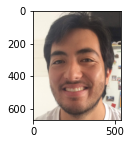
\includegraphics{output_32_0}
    \end{center}
    { \hspace*{\fill} \\}
    
    \begin{Verbatim}[commandchars=\\\{\}]
True identity: Marcelo

Test 1
    \end{Verbatim}

    \begin{Verbatim}[commandchars=\\\{\}]
System: What is your identity?
User: Marcelo
    \end{Verbatim}

    \begin{Verbatim}[commandchars=\\\{\}]
System: Verification succeeded (Distance = 0.57)

Test 2
    \end{Verbatim}

    \begin{Verbatim}[commandchars=\\\{\}]
System: What is your identity?
User: Michal
    \end{Verbatim}

    \begin{Verbatim}[commandchars=\\\{\}]
System: Verification failed (Distance = 0.93)


    \end{Verbatim}

    \begin{center}
    
\includegraphics{output_32_6}
    \end{center}
    { \hspace*{\fill} \\}
    
    \begin{Verbatim}[commandchars=\\\{\}]
True identity: Jola

Test 1
    \end{Verbatim}

    \begin{Verbatim}[commandchars=\\\{\}]
System: What is your identity?
User: Jola
    \end{Verbatim}

    \begin{Verbatim}[commandchars=\\\{\}]
System: Verification succeeded (Distance = 0.56)

Test 2
    \end{Verbatim}

    \begin{Verbatim}[commandchars=\\\{\}]
System: What is your identity?
User: Ala
    \end{Verbatim}

    \begin{Verbatim}[commandchars=\\\{\}]
System: Verification failed (Distance = 0.71)


    \end{Verbatim}

    \begin{center}
    
\includegraphics{output_32_12}
    \end{center}
    { \hspace*{\fill} \\}
    
    \begin{Verbatim}[commandchars=\\\{\}]
True identity: Marek

Test 1
    \end{Verbatim}

    \begin{Verbatim}[commandchars=\\\{\}]
System: What is your identity?
User: Marek
    \end{Verbatim}

    \begin{Verbatim}[commandchars=\\\{\}]
System: Verification succeeded (Distance = 0.59)

Test 2
    \end{Verbatim}

    \begin{Verbatim}[commandchars=\\\{\}]
System: What is your identity?
User: Michal
    \end{Verbatim}

    \begin{Verbatim}[commandchars=\\\{\}]
System: Verification failed (Distance = 0.90)


    \end{Verbatim}

    \begin{center}
    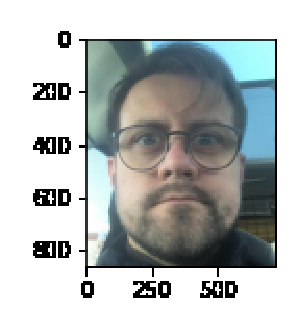
\includegraphics{output_32_18}
    \end{center}
    { \hspace*{\fill} \\}
    
    \begin{Verbatim}[commandchars=\\\{\}]
True identity: Michal

Test 1
    \end{Verbatim}

    \begin{Verbatim}[commandchars=\\\{\}]
System: What is your identity?
User: Michal
    \end{Verbatim}

    \begin{Verbatim}[commandchars=\\\{\}]
System: Verification succeeded (Distance = 0.56)

Test 2
    \end{Verbatim}

    \begin{Verbatim}[commandchars=\\\{\}]
System: What is your identity?
User: Marek
    \end{Verbatim}

    \begin{Verbatim}[commandchars=\\\{\}]
System: Verification failed (Distance = 0.72)


    \end{Verbatim}

    \begin{center}
    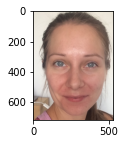
\includegraphics{output_32_24}
    \end{center}
    { \hspace*{\fill} \\}
    
    \begin{Verbatim}[commandchars=\\\{\}]
True identity: Ala

Test 1
    \end{Verbatim}

    \begin{Verbatim}[commandchars=\\\{\}]
System: What is your identity?
User: Ala
    \end{Verbatim}

    \begin{Verbatim}[commandchars=\\\{\}]
System: Verification succeeded (Distance = 0.60)

Test 2
    \end{Verbatim}

    \begin{Verbatim}[commandchars=\\\{\}]
System: What is your identity?
User: Jola
    \end{Verbatim}

    \begin{Verbatim}[commandchars=\\\{\}]
System: Verification failed (Distance = 0.69)


    \end{Verbatim}

    \hypertarget{face-recognition}{%
\paragraph{Face recognition}\label{face-recognition}}

    \begin{tcolorbox}[breakable, size=fbox, boxrule=1pt, pad at break*=1mm,colback=cellbackground, colframe=cellborder]
\prompt{In}{incolor}{21}{\boxspacing}
\begin{Verbatim}[commandchars=\\\{\}]
\PY{k}{def} \PY{n+nf}{recognize}\PY{p}{(}\PY{n}{image\PYZus{}path}\PY{p}{,} \PY{n}{database}\PY{p}{)}\PY{p}{:}
    
    \PY{c+c1}{\PYZsh{} Encode the input image}
    \PY{n}{encoding} \PY{o}{=} \PY{n}{encode}\PY{p}{(}\PY{n}{image\PYZus{}path}\PY{p}{)}
    
    \PY{c+c1}{\PYZsh{} Initialize min\PYZus{}dist to a large number}
    \PY{n}{min\PYZus{}dist} \PY{o}{=} \PY{l+m+mi}{100}
    
    \PY{k}{for} \PY{p}{(}\PY{n}{name}\PY{p}{,} \PY{n}{db\PYZus{}enc}\PY{p}{)} \PY{o+ow}{in} \PY{n}{database}\PY{o}{.}\PY{n}{items}\PY{p}{(}\PY{p}{)}\PY{p}{:}
        
        \PY{c+c1}{\PYZsh{} Calculate L2 distance between encoding to recognize and current encoding from the database }
        \PY{k}{for} \PY{n}{each} \PY{o+ow}{in} \PY{n}{db\PYZus{}enc}\PY{p}{:}
            
            \PY{n}{dist} \PY{o}{=} \PY{n}{np}\PY{o}{.}\PY{n}{linalg}\PY{o}{.}\PY{n}{norm}\PY{p}{(}\PY{n}{encoding} \PY{o}{\PYZhy{}} \PY{n}{each}\PY{p}{)}
            
\PY{c+c1}{\PYZsh{}             print(\PYZsq{}\PYZpc{}s Distance: \PYZpc{}.2f\PYZsq{} \PYZpc{} (name, dist))}
            
            \PY{k}{if} \PY{n}{dist} \PY{o}{\PYZlt{}} \PY{n}{min\PYZus{}dist}\PY{p}{:}
                \PY{n}{min\PYZus{}dist} \PY{o}{=} \PY{n}{dist}
                \PY{n}{identity} \PY{o}{=} \PY{n}{name}
                
    \PY{c+c1}{\PYZsh{} Display predicted identity}
    \PY{n+nb}{print}\PY{p}{(}\PY{l+s+s1}{\PYZsq{}}\PY{l+s+s1}{Prediction: }\PY{l+s+si}{\PYZpc{}s}\PY{l+s+s1}{ }\PY{l+s+se}{\PYZbs{}n}\PY{l+s+s1}{Distance: }\PY{l+s+si}{\PYZpc{}.2f}\PY{l+s+se}{\PYZbs{}n}\PY{l+s+s1}{\PYZsq{}} \PY{o}{\PYZpc{}} \PY{p}{(}\PY{n}{identity}\PY{p}{,} \PY{n}{min\PYZus{}dist}\PY{p}{)}\PY{p}{)}
    
    \PY{k}{return} \PY{n}{min\PYZus{}dist}\PY{p}{,} \PY{n}{identity} 
\end{Verbatim}
\end{tcolorbox}

    \begin{tcolorbox}[breakable, size=fbox, boxrule=1pt, pad at break*=1mm,colback=cellbackground, colframe=cellborder]
\prompt{In}{incolor}{22}{\boxspacing}
\begin{Verbatim}[commandchars=\\\{\}]
\PY{n}{test\PYZus{}dir} \PY{o}{=} \PY{l+s+s1}{\PYZsq{}}\PY{l+s+s1}{./test}\PY{l+s+s1}{\PYZsq{}}
\PY{n}{images} \PY{o}{=} \PY{n+nb}{filter}\PY{p}{(}\PY{k}{lambda} \PY{n}{f}\PY{p}{:} \PY{o+ow}{not} \PY{n}{f}\PY{o}{.}\PY{n}{startswith}\PY{p}{(}\PY{l+s+s1}{\PYZsq{}}\PY{l+s+s1}{.}\PY{l+s+s1}{\PYZsq{}}\PY{p}{)}\PY{p}{,} \PY{n}{os}\PY{o}{.}\PY{n}{listdir}\PY{p}{(}\PY{n}{test\PYZus{}dir}\PY{p}{)}\PY{p}{)}

\PY{k}{for} \PY{n}{image} \PY{o+ow}{in} \PY{n}{images}\PY{p}{:}
    
    \PY{n}{img\PYZus{}path} \PY{o}{=} \PY{n}{os}\PY{o}{.}\PY{n}{path}\PY{o}{.}\PY{n}{join}\PY{p}{(}\PY{n}{test\PYZus{}dir}\PY{p}{,} \PY{n}{image}\PY{p}{)}

    \PY{c+c1}{\PYZsh{} Load image }
    \PY{n}{load\PYZus{}image}\PY{p}{(}\PY{n}{image\PYZus{}path}\PY{p}{)}
    
    \PY{c+c1}{\PYZsh{} Recognize a person }
    \PY{n}{min\PYZus{}dist}\PY{p}{,} \PY{n}{identity} \PY{o}{=} \PY{n}{recognize}\PY{p}{(}\PY{n}{img\PYZus{}path}\PY{p}{,} \PY{n}{database}\PY{p}{)}
\end{Verbatim}
\end{tcolorbox}

    \begin{center}
    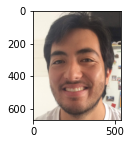
\includegraphics{output_35_0}
    \end{center}
    { \hspace*{\fill} \\}
    
    \begin{Verbatim}[commandchars=\\\{\}]
True identity: Marcelo
Prediction: Marcelo
Distance: 0.57

    \end{Verbatim}

    \begin{center}
    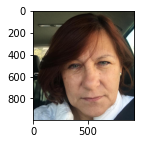
\includegraphics{output_35_2}
    \end{center}
    { \hspace*{\fill} \\}
    
    \begin{Verbatim}[commandchars=\\\{\}]
True identity: Jola
Prediction: Jola
Distance: 0.56

    \end{Verbatim}

    \begin{center}
    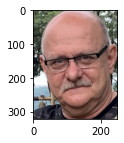
\includegraphics{output_35_4}
    \end{center}
    { \hspace*{\fill} \\}
    
    \begin{Verbatim}[commandchars=\\\{\}]
True identity: Marek
Prediction: Marek
Distance: 0.59

    \end{Verbatim}

    \begin{center}
    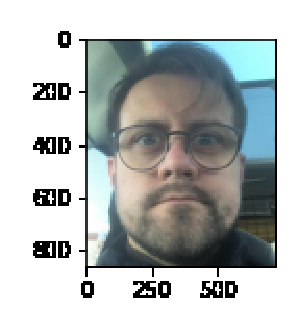
\includegraphics{output_35_6}
    \end{center}
    { \hspace*{\fill} \\}
    
    \begin{Verbatim}[commandchars=\\\{\}]
True identity: Michal
Prediction: Michal
Distance: 0.56

    \end{Verbatim}

    \begin{center}
    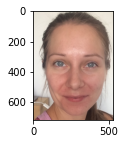
\includegraphics{output_35_8}
    \end{center}
    { \hspace*{\fill} \\}
    
    \begin{Verbatim}[commandchars=\\\{\}]
True identity: Ala
Prediction: Ala
Distance: 0.60

    \end{Verbatim}

    \begin{tcolorbox}[breakable, size=fbox, boxrule=1pt, pad at break*=1mm,colback=cellbackground, colframe=cellborder]
\prompt{In}{incolor}{ }{\boxspacing}
\begin{Verbatim}[commandchars=\\\{\}]

\end{Verbatim}
\end{tcolorbox}


    % Add a bibliography block to the postdoc
    
    
    
\end{document}
